%% LyX 1.5.6 created this file.  For more info, see http://www.lyx.org/.
%% Do not edit unless you really know what you are doing.
\documentclass[oneside,spanish,english]{book}
\usepackage[T1]{fontenc}
\usepackage[latin9]{inputenc}
\usepackage{geometry}
\geometry{verbose,letterpaper,tmargin=5cm,bmargin=3cm,lmargin=3cm,rmargin=3cm,headheight=5cm,headsep=1cm}
\pagestyle{headings}
\usepackage{array}
\usepackage{verbatim}
\usepackage{longtable}
\usepackage{varioref}
\usepackage{float}
\usepackage{amsmath}
\usepackage{color}
\usepackage{graphicx}
\usepackage{amssymb}

\makeatletter

%%%%%%%%%%%%%%%%%%%%%%%%%%%%%% LyX specific LaTeX commands.
\newcommand{\noun}[1]{\textsc{#1}}
%% Because html converters don't know tabularnewline
\providecommand{\tabularnewline}{\\}

%%%%%%%%%%%%%%%%%%%%%%%%%%%%%% User specified LaTeX commands.
\renewcommand\[{\begin{equation}}
\renewcommand\]{\end{equation}} 

\makeatother

\usepackage{babel}
\deactivatetilden

\begin{document}

\title{Paralell Training of Linear Transductive {SVM}s for Automated Text
Categorization}


\author{ \\ \\ \\  
 Miguel Fernando Cabrera Granados\\mfcabrer@unal.edu.co
\\ \\ \\ \\ \\ \\
Advisor\\
Jairo Jos\'{e} Espinosa  \\ \\ \\ \\ \\
Presented in Partial Fulfillment \\ 
of the Requirements \\
for the Degree of \\
Ingeniero de Sistemas e Inform\'{a}tica \\ \\ \\ 
Escuela de Sistemas - Facultad de Minas\\
Universidad Nacional de Colombia - Sede Medell\'{i}n\\}

\maketitle

\section*{Resumen}

\selectlanguage{spanish}%
Maquinas de Soporte Vectoriales Transductivos (TSVM) han mostrado
mejoras en tareas de clasificaci�n donde las caracter�sticas presentan
co-ocurrencia y los ejemplos de entrenamiento son pocos en comparaci�n
con los datos disponible como es com�n en problemas de categorizaci�n
de textos (TC). Aunque la naturaleza del algoritmo de TSVM descrito
por Joachims hace dif�cil que sea tan veloz como una SVM regular,
la paralelizaci�n de este algoritmo es interesante cuando las ganancias
en la efectividad de clasificaci�n es crucial. Resolver el algoritmo
de TSVM requiere la soluci�n de m�ltiples problemas de programaci�n
cuadr�tica que generalmente escalan a $O(n^{3})$. Aqu� describimos
una implementaci�n de un TSVM para problemas de clasificaci�n binaria
usando una arquitectura paralela que busca mejorar los tiempos de
computo necesarios mientras preserva la efectividad de la clasificaci�n.
Para lograr este objetivo adaptamos la arquitectura en cascada desarrollada
por Graf et al. para SVM regulares. La uni�n de estas estrategias
produjo una implementaci�n que es de 2 a 7 veces mas r�pida que una
TSVM regular para un problema de TC de 2.000 vectores y mas de 30.000
caracter�sticas.

\textbf{Palabras Clave}: Maquinas de Soporte Vectorial,Aprendizaje
de M�quina, IA, Clasificaci�n, Recuperaci�n de Informaci�n, Paralelizaci�n.

\selectlanguage{english}%
\newpage{}


\section*{Abstract}

Transductive Support Vector Machines (TSVM) have shown improvements
on classification tasks such as Text Categorization (TC), where the
features present co-occurrence and the training samples are few in
comparison with the data available . Although the nature of the TSVM
algorithm as described by Joachim makes is difficult to be as fast
as a regular SVM, the parallelization of this algorithm is interesting
when the gains in classification performance are crucial. Solving
TSVM algorithm requires the solution of multiple quadratic programming
problems that generally scales to $O(n^{3})$. We describe the implementation
of a TSVM Solver for 2-class problem using a parallel architecture
which aims to improve the necessary computation times while preserving
the classification performance. For this purpose we adapt the parallel
cascade architecture for regular SVM described by Graf et al.%
\begin{comment}
We also experiment with an alternative heuristic for choice of the
$C*$ parameter for the TSVM problem
\end{comment}
{}. This strategy produced an implementation that is 2x - 7x faster
than a regular TSVM for a TC problem of 2,000 vectors and more than
30,000 features.

\textbf{Keywords}: SVM, Classification, Machine Learning, Algorithm,
Parallel, Infomrmation Retrieval.

\tableofcontents{}




\chapter{Overview}


\section{Introduction}

Text classification is a key aspect of text filtering, document management
and retrieval tasks. Besides basic document classification for some
kind of digital library, many problems can be seen as instances of
the Text Categorization (TC) problem . Spam detection, Web search
improvement and automated metadata generation are just a few examples
of this \cite{Sebastiani02}.  Some of those tasks can be achieved
by human beings, but a manual classification is at best expensive
and practically impossible for large amounts of documents found today
in modern information systems.

A TC technique uses example documents that have been previously categorized
in classes by an authority in order to learn a model that, with an
associated error value, can automatically predict the class that the
authority would have given to future documents. 

Support Vector Machines \cite{Vapnik98} are powerful tools for classifying
large data sets, and due the nature of the classical text representation
models, it has been applied successfully in automated document classification
tasks \cite{Joachims98,Joachims99c}. An special type of SVM, based
on Transductive inference (TSVM), has demonstrated to be more effective
for document classification than the common inductive inference based
SVM \cite{Joachims99c}.

One characteristic of the SVM is that, in its formal definition, the
computation and memory storage requirements increase rapidly with
the number of training vectors. This is due the fact that the SVM
classification problem is a Quadratic Programming problem (QP) that
finds the support vectors in all training data set. Solvers of this
kind of problem generally scales to $O(n^{3})$ making it a very computationally
expensive problem.

One approach to cope with this limitation is to divide the problem
into chunks \cite{Joachims/99a,osunaetal97} and train those sub-problems.
Even with these optimizations, the problem still has large computational
requirements, and the required time to train grows sufficiently enough
for making it not useful for real-time training when using large data
sets. The implementation of Transductive inference for a SVM requires
to solve the same problem many times over generally large data sets,
until finding the optimal classifier. This makes the scaling problem
for Transductive SVM even more difficult, therefore, methods for optimizing
the training process need to be developed.

Taking advantage actual trends in processor technologies, where the
multi-core processor is becoming the norm \cite{Marowka07,1069628|Geer05}
parallel implementation of such algorithm along with other optimization
will help make the application of this technique practical in real
world situations. Also, as an extra motivation, empirical results
have showed that some parallel settings for SVM have achieved better
generalization than their classic counterparts for some problems \cite{citeulike:935557|Collobert2002}.

This work describes an implementation of a parallel SVM using the
cascade model described in \cite{GrafCBDV04} using a Transductive
learning algorithm. The first part, Overview, introduces the basic
concepts a Machine Learning, Information Retrieval and Text Categorization.
Later we describe the SVM algorithm and justify the reason of using
SVM for text classification over other techniques. In chapter \ref{cha:Experiments-and-Results}
we exhibit our experimental set-up and the show the analysis of the
results.


\section{Machine Learning}

Machine Learning (\noun{ML}) is concerned with the question of how
to construct computer programs that automatically improve with experience
\cite{Mitchell97}. The experience encountered by the computer program
are examples that it takes as input. In order to to develop such programs
\noun{ML} borrows concepts from many areas such Statistics, Information
Theory, Biology and Control Theory, furthermore, given the amount
of statistical based ML algorithms developed in the last years, many
scientists see ML as a crossroad between Statistics and Computer Science.

The learning problem is defined formally in \cite{Mitchell97} as
follows:

\begin{description}
\item [{Learning:}] A computer program is said to \emph{learn} from experience
$E$ with respect to some class of Task $T$ and performance measurer
$P$, if its performance at tasks in $T$, as measured by $P$ improves
with $E$. 
\end{description}
In other words, the program learns from an experience commonly represented
by a group of data belonging to a universe on which the result of
Task $T$ is known. Using this information the computer program tries
to generalize for over the available data, thus learning a representation
of the universe. 

The way in which an actual computer program realizes the task of learning
from the experience can different, there are several modes in which
the learning task can be accomplished \cite{citeulike:755348|Heibrich2001Lkernel}:

\begin{itemize}
\item \emph{Supervised Learning}: In which the program generates an internal
representation that maps inputs, to desired outputs. Classification
problems can be seen as an instance of this type of learning, where
the desired output is a binary value stating whether the input belongs
to a specific category.
\item \emph{Unsupervised Learning:} Combines both labeled and unlabeled
examples to generate the representation.
\item \emph{Reinforcement Learning}: In which the algorithm learns a policy
of how to act given an observation of the world.
\end{itemize}
Besides these three main ways of learning, there are others that can
be seen as variations of the ones mentioned above.

\begin{itemize}
\item \emph{Semi-supervised Learning}: Combines both labeled and unlabeled
examples to generate the representation.
\item \emph{Transductive Learning}: Similar to Semi-supervised Learning,
but does not explicitly construct a function: instead, tries to predict
new outputs based on training inputs, training outputs and test input
which are available while training. 
\end{itemize}
In this thesis we are going to use a restricted definition in order
to illustrate the concepts described above. In these pages machine
learning will refer to a generalized regression characterizing a set
of label events $\left\{ (x_{1},y_{1}),(x_{2},y_{2}),...,(x_{n},y_{n})\right\} $
with a function $\Phi:X\rightarrow Y$ from event to label . Many
researcher has used this setting with success \cite{Berger2001} .
The reader will notice the similarity between this definition and
the definition of text categorization described in section \vref{sec:Text-Categorization}. 

The question of how good the function $\Phi$ can generalize has spawned
an entire subfield of machine learning called computational learning
theory. Many of the techniques classified in this field have come
from development of frameworks in this particular subfield. These
frameworks generally don't state how good is going to perform an algorithm,
instead create a probabilistic bound to the performance.

 Some of techniques generally classified under ML are Artificial
Neural Networks, Genetics Algorithm, k-Nearest Neighbor, Bayesian
Networks and and Support Vector Machines (SVM) and has been successfully
applied to.




\section{Information Retrieval}



Information Retrieval (IR) is branch of computer science whose original
objective was to obtain information from generally large amounts of
data. Today modern IR deals with content-based document management
task, including document filtering, translation, summarization, question
answering among others. 

IR Systems makes large amounts of text accessible to people that need
the information. A user the approaches to the system with a vague
idea of what is looking for, so the goal of the system is to provide
the information required. The user provides generally provides some
information about what kind of documents is looking for, in the form
of keywords.

And information retrieval system comprises several modules, Figure
\ref{fig:ir-kelle} shows the basic scheme of work of a basic IR system. 

%
\begin{figure}[H]
\begin{centering}
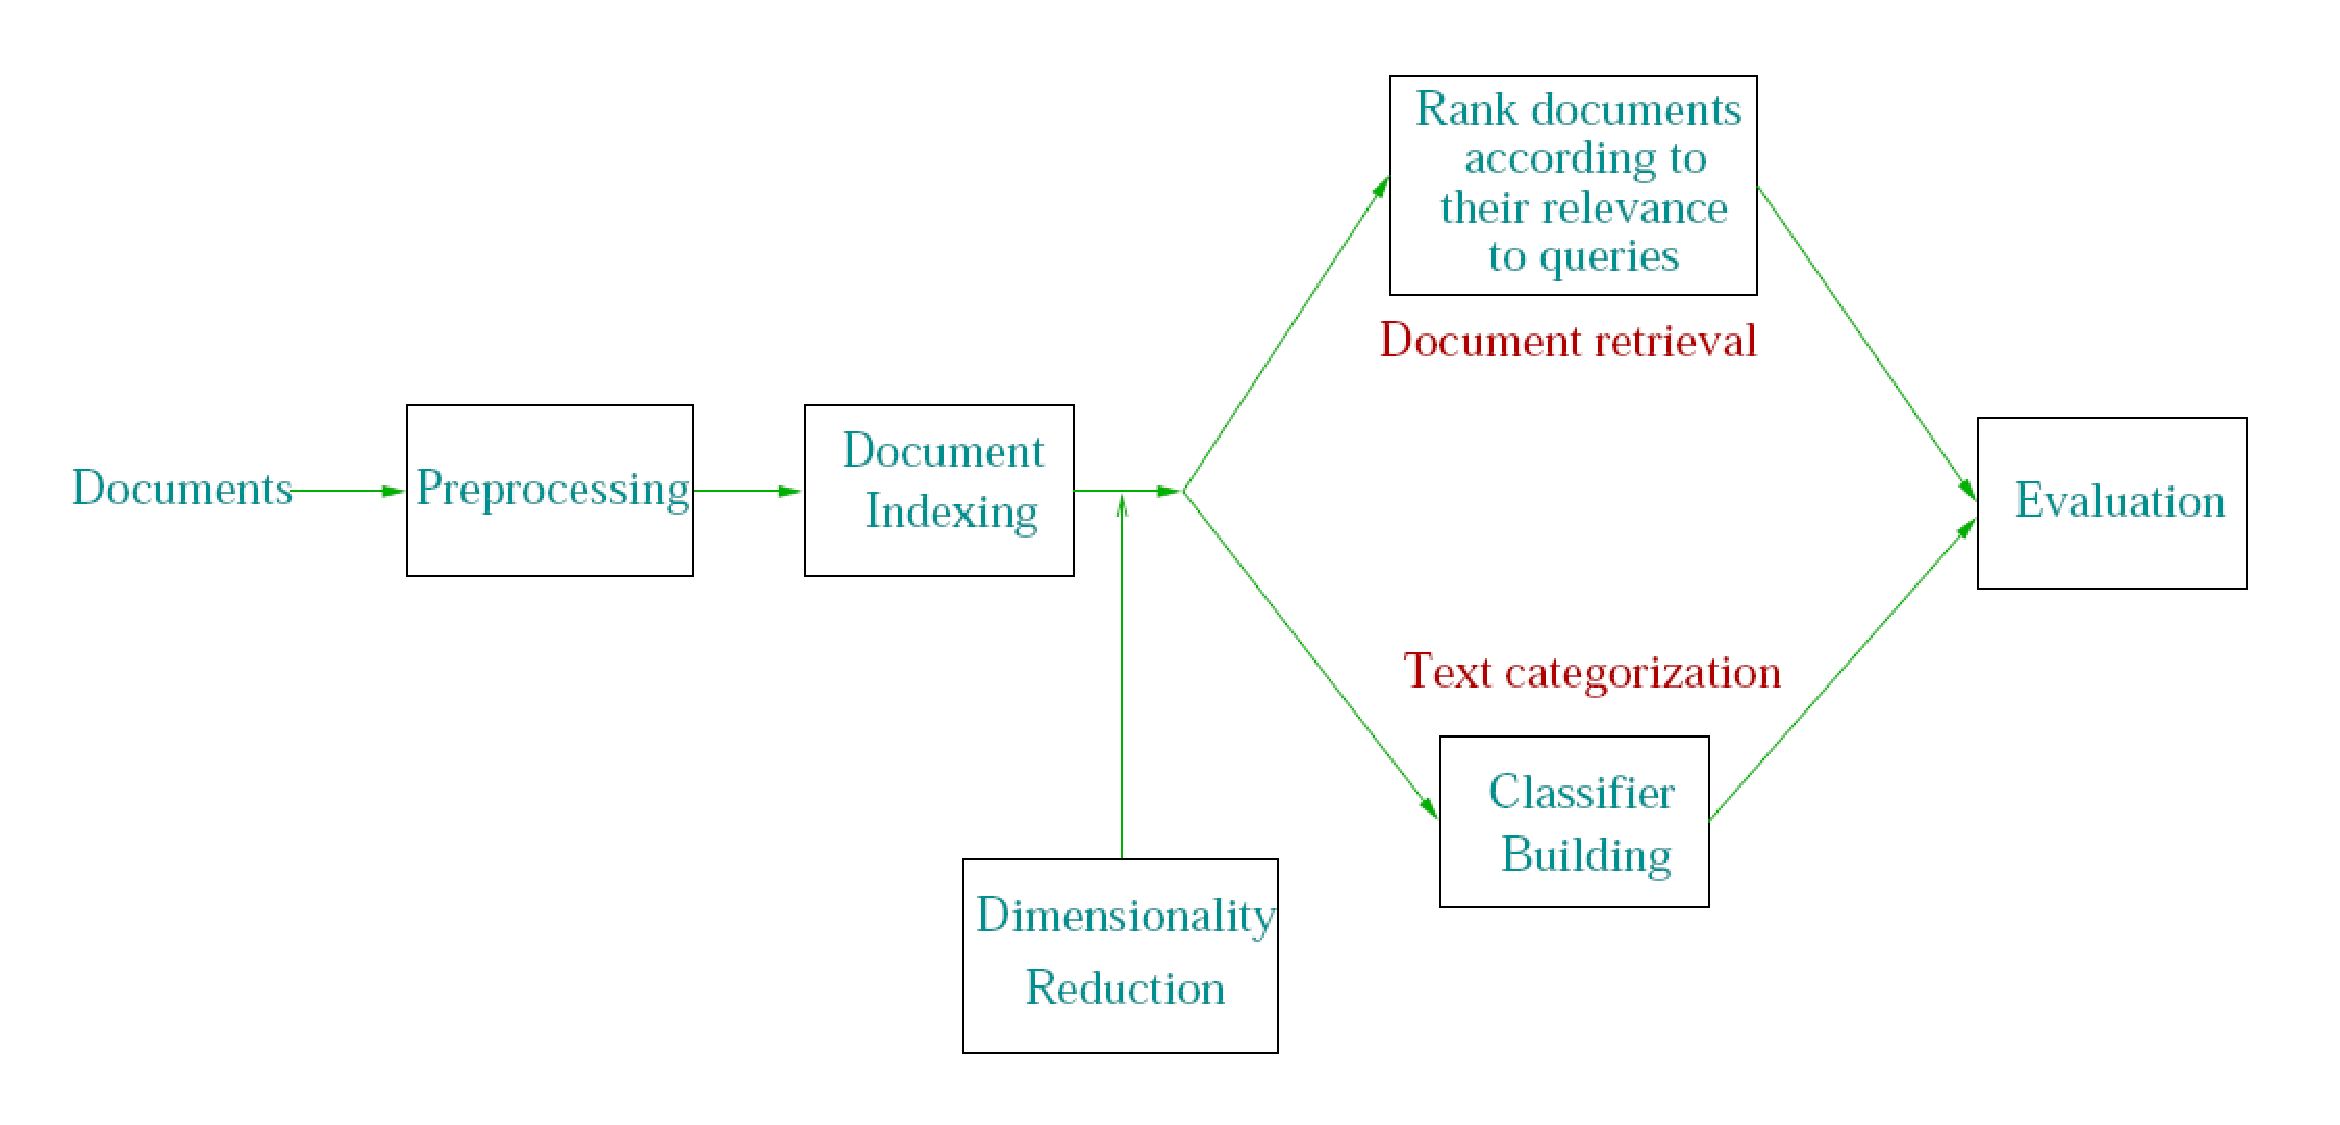
\includegraphics[scale=0.3]{images/keller-ir-diagram}
\par\end{centering}

\caption{Parts of an Information Retrieval System \label{fig:ir-kelle}}

\end{figure}


 

In today's information society where digital text is becoming more
and more available, boosted by the usage of the Internet and more
and more fast networks and larger capacities of storage, the need
of better information retrieval techniques becomes everyday more strong. 

%
\begin{comment}
Although IR task has been already automated only in the last decade
Machine Learning techniques has been applied to IR systems. ML techniques
have shown to be very useful even surpassing in performance classical
classification methods such as {}``ROCHIO'' algorithm. In the next
sections of the chapter we show how textual information is handled
and prepared for the Text Categorization task.
\end{comment}
{}


\subsection{Models of Text and Text Representation\label{sub:Models-of-Text}}

Usually in a digital library database a set of words that defines
the topics or the main characteristics of a document is manually defined.
The main objective of this is to help the search of the physical document
(e.g books, papers,etc.). This list of terms or keywords enables the
user to query documents related to one or more concepts. One of the
main problems of this is that only few keywords are associated with
a defined document, and generally this assignation is made at hand,
making it expensive and error prone. Generally this querying these
systems was limited to the numbers of keywords assigned and some metadata
like title, author and dates of publication, being the user unable
to query the whole document, making the retrieval task significantly
harder.

Nowadays in digital libraries and similar systems where the all the
text is available in digital form, automatic keyword extraction makes
sense because these keywords are tightly associated with the content.
This keywords are called indexes and the task of associating each
document with a set of keywords is called \emph{indexing}. 

Indexing is based is predefined group of keywords: the dictionary
or vocabulary. As mentioned above, in a digitalized text database
(also called a corpus) the dictionary is usually extracted from the
set of words present in the corpus, and the expensive manual indexing
can be avoided by representing the documents by the dictionary terms
they are made of. Given that all the full text is available for querying
it, now problem is to find the best way of representing the text in
order to extract the more important words, that is, the keywords that
define it. 

During the last few decades many representation forms have been developed
ranging from simple word appearance binary representation to a concept
\cite{deerwester90indexing}, probabilistic \cite{keller-theme} and
even Neural Networks \cite{DBLP:conf/icann/KellerB05} based ones. 

The most common approach to automatically extract the index terms
from a corpus is called vector space model \cite{361220}. In this
model each document $d$ is represents as a vector$(\theta_{1},...,\theta_{M})$
where $\theta_{j}$ is a function of the frequency in $d$ of the
$j^{th}$ word of a chosen dictionary $M$. 

Based in this definition various forms of $\theta(j)$have been defined:

\begin{description}
\item [{Binary}] In which $\theta_{j}$ is equal to 1 if the $j^{th}$
word appears in the document or 0 otherwise.
\item [{Frequency}] In which $\theta_{j}$ is equal to the number of times
$j^{th}$ word appears in the document.
\item [{\emph{tf-idf}}] In which $\theta_{j}$ is equal to the \emph{tf-idf}
formula:
\end{description}
\begin{equation}
\theta_{j}=tf_{j}(d)\centerdot log(\frac{N}{df_{j}}),\,\,\,\,\forall j\in\{1,\ldots,M\}\label{eq:tf-idf}\end{equation}


The equation \ref{eq:tf-idf} was defined proposed by Salton and Buckley
\cite{866292} and it is the more complex of the three. the $tf_{j}(d)$
(term frequency) is the number of times that the $j^{th}$ word appears
in the document $d$, $df_{j}$ is the number of documents the term
appears in all the corpus and $N$ is the total number of documents
in the corpus. The main reason behind this formulation is that in
the context of document retrieval it is considered that words appearing
too frequently across the corpus may not be discriminant, therefore
this formula gives more importance to terms appearing more frequently
in the documents while penalizing the ones that appears in to many
documents. The reader may have noticed that this representation of
text does not take into account the actual order of the words inside
the document, despite this, vector space model have performed well
and it still used with some variations in the majority of IR systems.





the vector space model representation described above may seem simplistic
in comparison with the more complex representation mentioned first,
nevertheless, it seems that for some tasks like text categorization,
the classical tf-idf works just well and more complex representations
of the text do not significantly affect the performance of the methods.

%
\begin{figure}
\begin{centering}
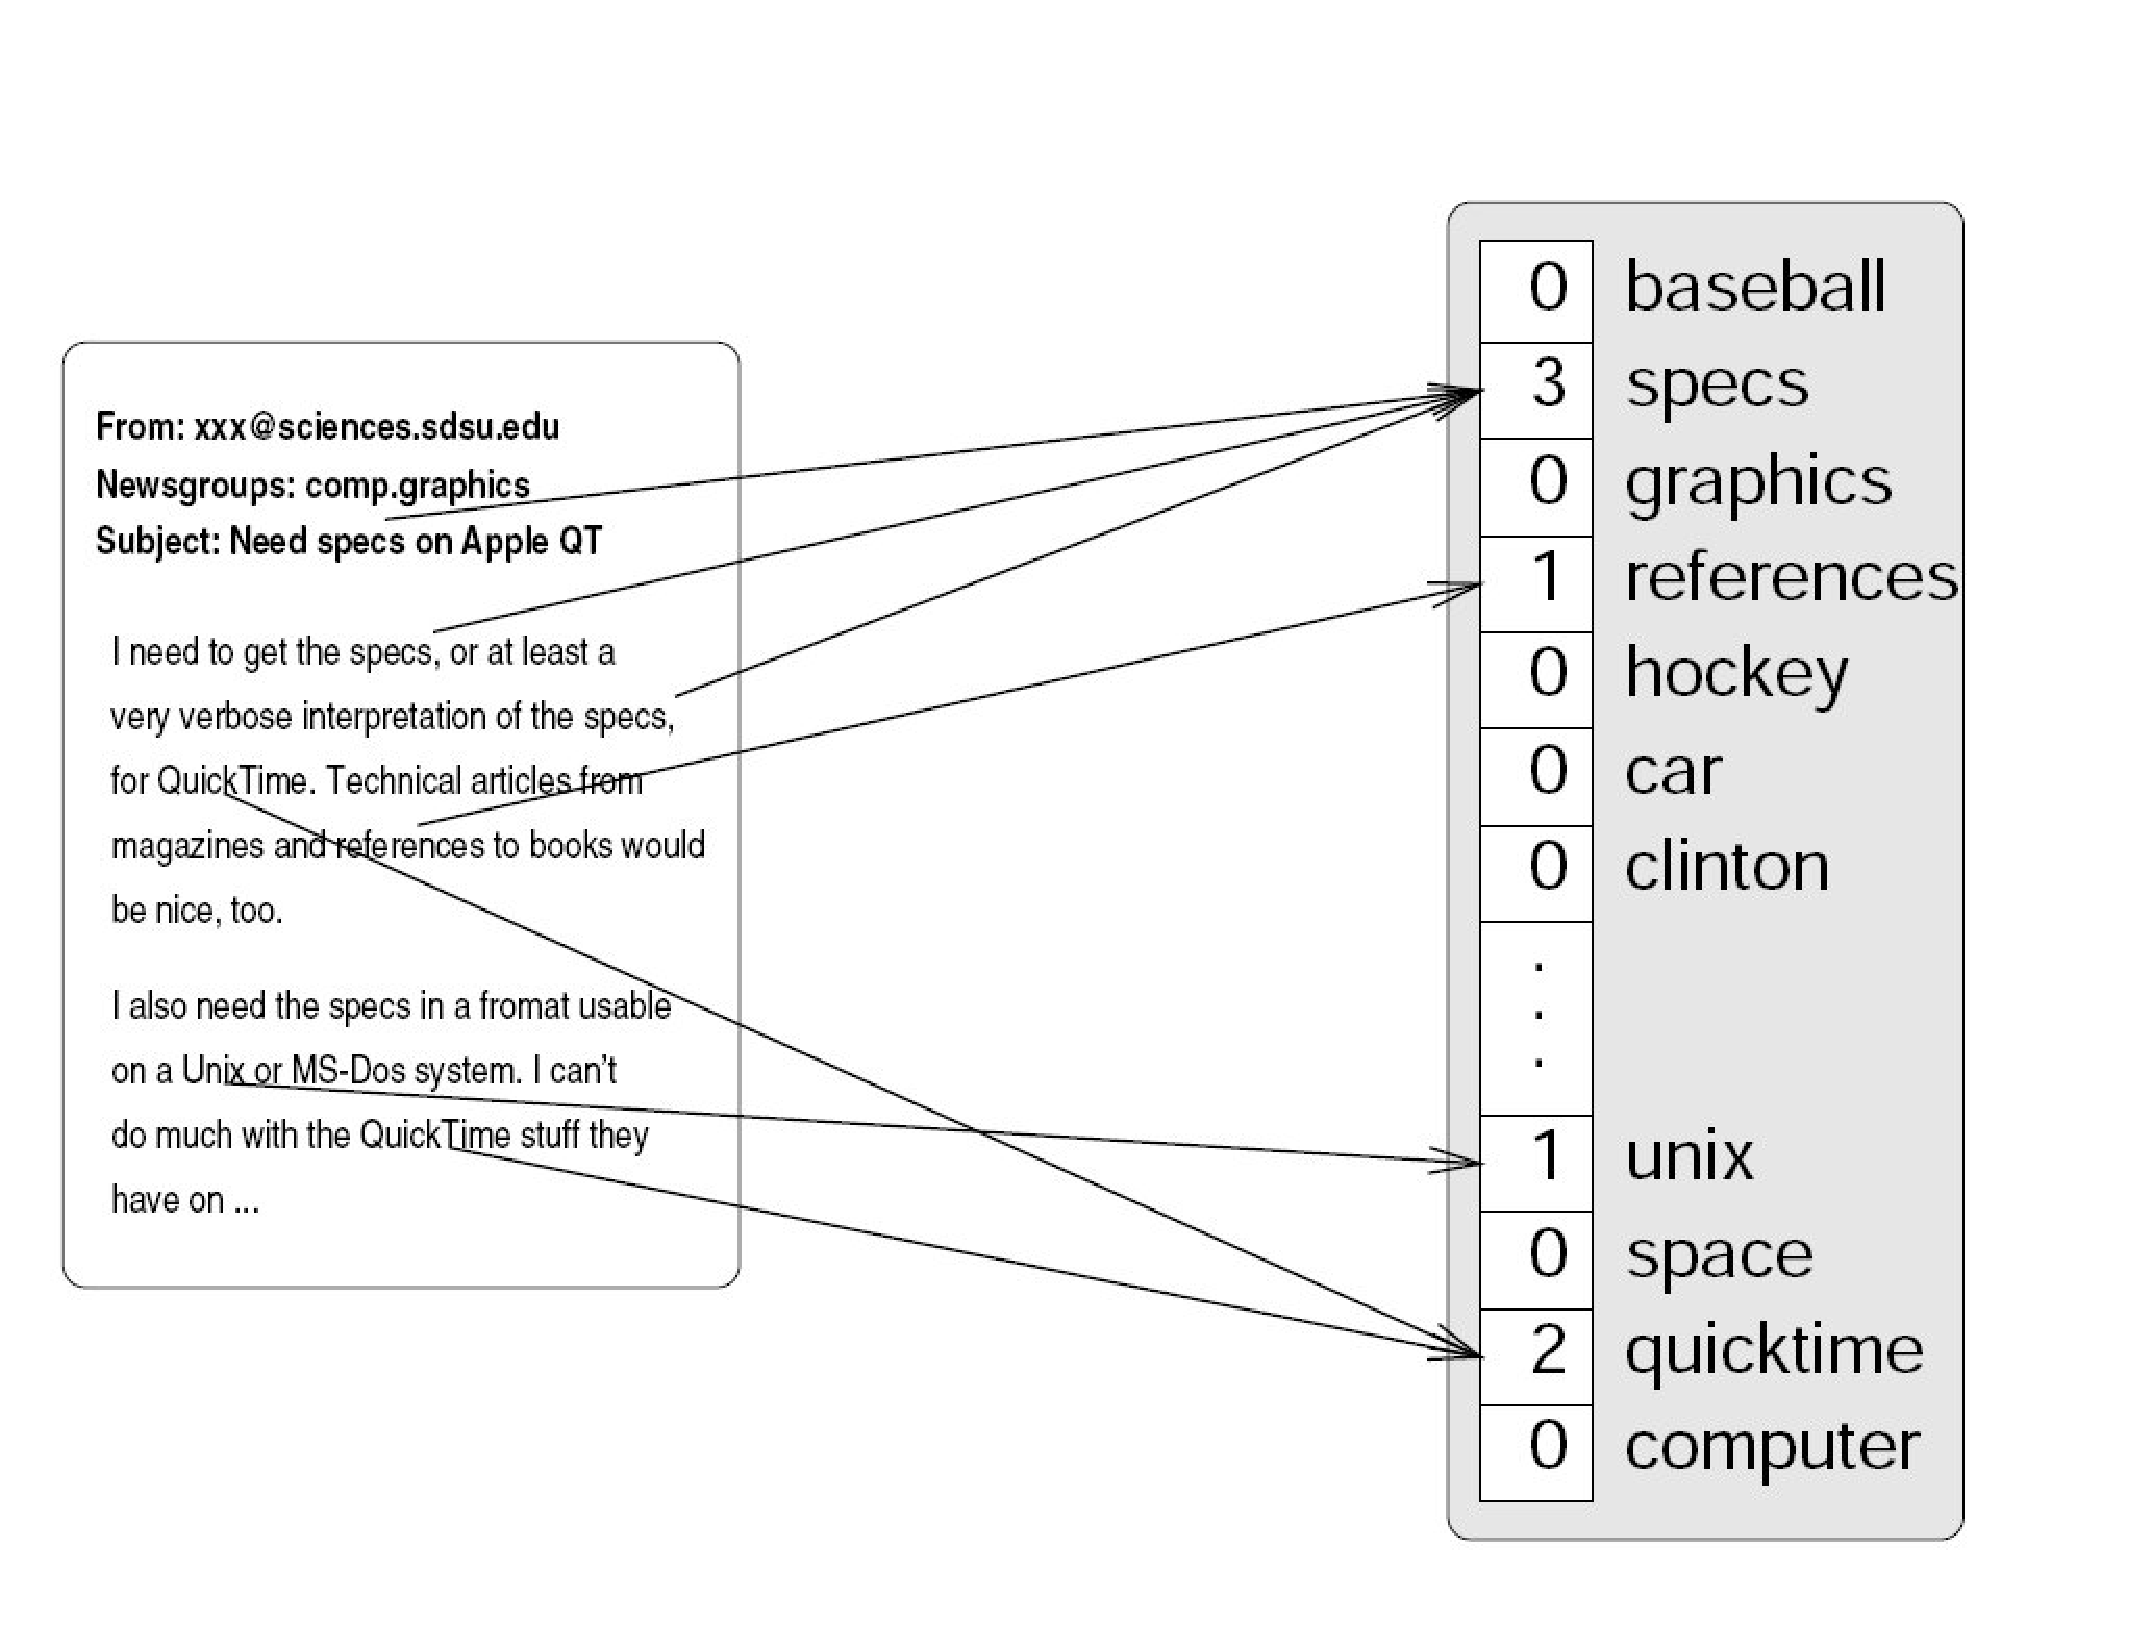
\includegraphics[scale=0.2]{images/joachims-text-vect}
\par\end{centering}

\caption{Representing text as a feature vector \cite{Joachims98}}

\end{figure}



\subsection{Feature Selection and Dimensionality Reduction\label{sub:Feature-Selection-and}}

Due to the fact that the representation of the text can have impact
in any retrieval task, any strategy to enhance the representation
of text should be studied. With the years, many techniques have been
developed in the field of Information Retrieval in order to get a
better performance on the representation of the text made. IR research
shows us that the word stems work well as representation units \cite{Joachims98}.
The word stemming process (sometimes called term conflation) consists
in removing the case and flection information from a word \cite{Porter80}.
For example words as {}``engine'', {}``engineer'', {}``engineering''
becomes the same term {}``engin''. Generally this techniques are
applied to the document before the transforming it into a term vector
representation, thus making the resulting document vector notably
smaller.

Another technique used to avoid unnecessary large feature vectors
is removed the so-called stop-words, or the words that for their common
use is known that are not significant for the text. Words like {}``and'',
{}``or'', {}``of'', etc are removed from the original text.

There are other approaches for selecting the most important features
other than the described above, these approaches try to select the
most important features (the {}``best'' words) from the dictionary
$M$, creating a subset $M0$, that used for document representation
provides better results. However, Joachims \cite{Joachims98} shows
that the {}``worst'' features still contain important information,
therefore suggest that all features should be selected, when it is
possible.


\section{Text Categorization\label{sec:Text-Categorization}}

The goal of text categorization (TC) is to automatically assign, for
each documents, categories selected among a predefined set. In opposition
to the machine learning typical multi-class classification task which
aims at attributing one class among the possible ones to each example,
documents in a text categorization task may belong to several categories.
Sebastiani \cite{Sebastiani02} formally defines TC as task of assigning
a Boolean to each pair $\left\langle d_{j},c_{j}\right\rangle \in\mathcal{D}\,\, x\,\mathcal{\, C}$
where $\mathcal{D}$ is a domain of documents and $\mathcal{C}=\{c_{1},\ldots,c_{|c|}\}$
is a set of predefined categories. a true value assigned to the pair
$\left\langle d_{j},c_{j}\right\rangle $ indicates the decision of
filling $d_{j}$ under category $c_{j}$, and a false value the decision
of not filling it under that category. More formally the task is to
approximate a unknown target function $\breve{\Phi}:\mathcal{D}\,\, x\,\mathcal{\, C}\rightarrow\{T,F\}$
using $\Phi:\mathcal{D}\,\, x\,\mathcal{\, C}\rightarrow\{T,F\}$
such that $\Phi$and $\breve{\Phi}$ {}``coincide as much as possible''
\cite{Sebastiani02}. 

A text categorization task can be performed in many ways, for instance
one might want to classify a document in just one category (single
label case or not overlapping categories) or from $0$ to $|\mathcal{C}|$
categories (multilabel case or overlapping categories). A special
case of single label TC is the binary TC in which each $d_{j}$ is
assigned to category $c_{i}$ or its complement $\widetilde{c}_{i}$. 

It is possible to perceive the multilabel case as different problem
but one can express the multilabeled TC task for a set of categories
$\mathcal{C}=\{c_{1},\ldots,c_{k}\}$ as a group of $k$ binary case
problems, this requires that categories be stochastic independent
or each other although some recent development in structured classification
\cite{Tsochantaridis/etal/05a} might be useful to tackle multilabel
interdependent TC task. In this work we are going to deal with binary
categorization tasks because as stated by Sebastiani \cite{Sebastiani02}
many important TC applications are in fact binary categorization problems
and moreover, as described above we can solve multilabel TC as many
binary TC task assuming independent categories, which is a valid assumption
for most of the problems. 

TC heavily relies on the models that have been developed for IR. the
reason of this is that TC is a content based document management task,
and such it shares many characteristics with other IR tasks such as
text search, specifically IR-style indexing using one of the models
mentioned in \ref{sub:Models-of-Text} and the evaluation of effectiveness
of the classifier using the measures described below.


\subsection{Performance Measures}

One question that arises after reading the definition of TC is how
to measure the how well the classifier function$\breve{\Phi}$ (the
approximation or hypothesis) matches the unknown target function $\Phi$
(effectiveness). This is generally measured in terms of the classic
IR metrics of precision $P$ and recall $R$ but adapted to the specific
case of TC. $P$ is defined as the probability that if a given a random
document $d_{x}$ is classified under the category $c_{i}$ the classification
is correct ($P(\breve{\Phi}(d_{x},c_{i})=T\,\,|\,\, P(\Phi(d_{x},c_{i})=T)$).
Analogously $R$ is defined as the probability that if a random document
$d_{x}$ is ought to be classified under $c_{i}$, this decision is
taken ($P(\Phi(d_{x},c_{i})=T\,\,|\,\, P(\breve{\Phi}(d_{x},c_{i})=T)$). 

In binary TC, with we can express the concepts of precision and recall
mathematically using the numbers of true positive ($TP$), false positive
($FP$), true negative ($TN$) and false negative ($TN$) documents
classified. The true of false value means that the classification
was performed correctly or not, and the positive or negative define
whether it belonged to the evaluated category or not. Using these
definitions we can write precision $P$ and recall $R$ as:

\begin{eqnarray*}
P=\frac{TP}{TP+FP} & ,\, & R=\frac{TP}{TP+FN}\end{eqnarray*}


For multilabel classification this only would be local measures for
a single category c, in that case the local measures are averaged
using different methods such as \emph{microaveraging }and \emph{macroaveraging}
\cite{Sebastiani02}.

The values of precision and recall for TC vary in an inverse relation,
for that reason many articles about TC uses break-even point of $P$
and $R$ \cite{Joachims98,DumaisPHS98,Lewis_et_al_2004} which generally
implies to modify in some degree the hypothesis. Another approach
is to use the $F1$ measure \cite{citeulike:543360,Manevitz_et_al2002,112471}
which combines both precision and recall and is defined as:

\[
F1=\frac{2RP}{P+R}\]


This implies that $F1$, like $P$ and $R$ is bounded by 1 and the
best results under this measure are the higher values. 


\subsection{Applications of Automated Text Categorization}

One can think that the application of TC are somewhat limited to automated
document classification but many problems can be seen as special instances
of TC, Sebastini \cite{Sebastiani02} list some of them:


\subsubsection{Document Organization}

Maybe the first application that comes to the mind when thinking in
TC. Indexing with a controlled vocabulary is an instance of this problem
that can be solved with TC techniques. Also any kind of document organization
and filing such personal information or enterprise data organization
can be viewed as instances of this problem. For example one can think
in newspaper ads and the categories in which they should be classified,
this is generally done at hand but can be addressed with many of the
existing TC techniques. Other applications includes automatic patent
classification, automatic news classification under topic sections
(e.g Politics, Lifestyles, Sports, etc.).


\subsubsection{Text Filtering}

Text filtering is the activity of classifying a stream of incoming
documents dispatched in an asynchronous way by an information producer
to an information consumer \cite{Sebastiani02}, for example a newsfeed
where the producer is the news agency and the consumer is the producer
is the newspaper or a RSS feed where the producer is the website and
the consumer the individual users that syndicate the feed.


\subsubsection*{Automated Metadata Extraction}

In digital libraries, one is usually interested in tagging documents
by metadata that describes them under a variety of aspects (e.g.,
creation date, document type or format, availability, etc.). Some
of this metadata is thematic, that is, its role is to describe the
semantics of the document by means of bibliographic codes, key words
or key phrases. The generation of this metadata may thus be viewed
as a problem of document indexing with controlled dictionary, and
thus tackled by means of TC techniques.


\subsection{Machine Learning Text Categorization Techniques}

The construction of Text Classifiers using an inductive approach have
been tackled using different strategies, we are going to mention some
of the most popular approaches included the technique that we will
use through the rest of the text. There are two ways of classify a
item in a category, the {}``hard'' (automated) way which is basically
a binary approach and the {}``soft'' o ranking (semi automated).

A ranking classifier is generally accomplished defining a function
$CSV_{i}\,:\, D\rightarrow[0,1]$ that, given a document $d_{j}$returns
a categorization status value for the $c_{i}$ category (how much
the classier believes that the document belong to that category) whereas
the hard approach only accepts or reject a document under a defined
category.


\subsubsection*{Probabilistic Classifiers}

The probabilistic based text classifiers are very popular, they see
the $CSV_{i}(d_{j})$ in terms of $P(c_{i}|d_{j})$. In other words,
the probability that a document represented by vector $d_{j}=(w_{1j,}w_{2j},\ldots,w_{|M|j})$
(that can be binary or weighted as mentioned in section \ref{sub:Models-of-Text})
belongs $c_{i}$ and computes this probability by application of the
Bayes theorem. 


\subsubsection*{Decision Trees Classifiers}

Probabilistic classifier are quantitative, that is, numeric in nature.
This kind of methods are often criticized since, effective as they
may be, they are no easily interpretable by humans. Symbolic (non-numeric)
techniques no suffer of this problem. In this category decision trees
learning is one of the most important example. A decision tree (DT)
text classifier \cite{Mitchell97,Sebastiani02} is a tree in which
internal nodes are labeled by terms, branches departing from them
are labeled by tests on the weight that the term has in the test document,
and leaf are labeled by categories. This kind of classifier categorizes
a test document $d_{j}$ by recursively testing for the weights that
the terms labeling internal nodes have in vector $\overrightarrow{d_{j}}$
, until a leaf node is reached. the label of this node is then assigned
to $d_{j}$. 


\subsubsection*{Support Vector Machines}

Support Vector Machine (SVM) method has been introduced in TC by Joachims
\cite{Joachims98,Joachims99c} and has been user by others in their
experiments with good results \cite{DumaisPHS98,Lewis_et_al_2004,112471}.
Basically SVM tries to find among all the surfaces $\sigma_{1,}\sigma_{2,}\ldots$
in a $|T|$-dimensional space that separate the positive from the
negative training examples (decision surface). This is done by finding
the decision surface with the widest margin of separation. How is
this accomplished and how can be applied to TC will be discussed in
depth in chapter \ref{cha:Text-Categorization-With}.


\section{Parallel Machine Learning\label{sec:Paralell-Machine-Learning}}

Only recently the topic of parallel implementation of machine learning
algorithms have come to importance, although it is rarely addressed
at major machine learning conferences, many factors points out that
the importance of this factor will increase. In his popular weblog%
\footnote{Machine Learning (Theory) - http://hunch.net/%
} John Langford%
\footnote{http://hunch.net/\textasciitilde{}jl/%
} describes the main tendencies of computation that impulse the necessity
of parallel implementation of machine learning algorithms:

\begin{enumerate}
\item Larger data sets available due to the availability of more sensors
on the Internet, making processor power a need in other to handle
these large amounts of information.
\item Serial processor speedups are stalled as the result of no having the
ability to drive chips at ever higher clock rates without excessively
increasing the cost. The new tendency for improving processor speed
is to have more cores per processor \cite{1069628|Geer05}, that is,
creating multicore processors, for example, IBM cell processor%
\footnote{http://www.research.ibm.com/cell/%
} has 9 cores.
\end{enumerate}
In addition, since 2005 there is low-cost parallel hardware aimed
to desktop users \cite{Marowka07} making even more important to take
advantage of this architecture and learn to use it the best way. 

With all these precedents the following question arises: how take
advantage of this trend and use all the parallel computing power of
new processor for solving machine learning problems? We are in the
beginning of the multicore era and there is no easy answer to this
question, mostly because there is not even an unified general approach
to take advantage of this architecture, although some basic strategies
can be described.

The basic approach is to run the same algorithm with different parameters
on different processors. Cluster software like Open Mosix, Condor
might be used in this situation. As noticed by Langford, this particular
approach does not speed up the run of a particular machine learning
algorithm. Other approaches includes the decomposition of the algorithm
into statistical queries \cite{167200} and parallelize the queries
over the the samples, for example using map-reduce \cite{conf/nips/ChuKLYBNO06}.
The last and most difficult way is to develop fine-grained parallelism,
which is the way brain actually works. 

We have discussed the evident speed gain using parallel methods for
running but the question whether the a parallel algorithm fine-grained
parallelize implementation can achieve better performance is still
unanswered. Another question that arises is if there are methods that
not necessarily incur in the complexity of dissecting a specific algorithm
and then paralleling and still harness parallel architectures. Graf
et Al. \cite{GrafCBDV04} presents the Cascade SVM, an approach for
parallelize the SVM without modifying the SVM problem at all but using
a pyramid-like array of SVM subproblem that are joined in each level
until a the solution is found. This approach is chosen for the experiments
of this work and will be discussed in depth in chapter \ref{cha:Experiments-and-Results}


\chapter{Text Categorization With SVM\label{cha:Text-Categorization-With}}


\section{Support Vector Machines}

Support Vector Machines (SVMs) \cite{Vapnik98} are powerful classification
and regression tools that have been widely applied in the solutions
of many problem, generally yielding comparable or even better performance
that other algorithms. 

The SVM algorithm is based on the concept of VC Dimension\cite{vapnik71uniform}
and on the principle of structural risk minimization developed by
Vapnik \cite{Vapnik99,vapnik71uniform}. Roughly, the VC dimension
is a metric of how complex a classifier machine is, complex classifier
has more capacity to fit the training data, thus, overfitting is more
likely to occur, therefore, is preferred a classifier with minimum
VC Dimension. 

The basic idea of empirical risk minimization principle is to find
an hypothesis $s$ from an hypothesis space $S$ for which the lowest
probability of error is guaranteed for a given set of training examples. 

For linear classification problems this is equivalent to find the
discrimination function that maximizes the distances within the classes,
assuring the lowest probability of error\cite{citeulike:368926|Haykin1998}.
The aim of the Support Vector classification is to devise a computationally
efficient way of learning the optimal separating hyperplanes in high
dimensional feature space \cite{citeulike:114719|Cristianini2000introSVM},



\subsection{Finding the Optimal Hyperplane}

Let us consider a training sample $\{(x_{i},y_{i})\}_{i=1}^{N}$,
where x is a point in $\mathbb{R}^{n}$ that belongs to the group
of training examples or input patterns for $i$th example and $d_{i}$
is the corresponded, desired response. In this case we are gonna simplifier
the setting by stating that $d_{i}$ can only take two values $\{+1,-1\}$
for the positive and negative classification case respectively. This
is case of a binary classification problem, for a multiclass classification
problem, we can transform it into different binary classification
ones. We also assume that the class represented by $y_{i}=\{+1,-1\}$
are linearly separable. The equation of a decision hyperplane that
separates the data is:

\begin{equation}
w^{T}x+b=0\label{eq:}\end{equation}


%
\begin{figure}
\begin{centering}
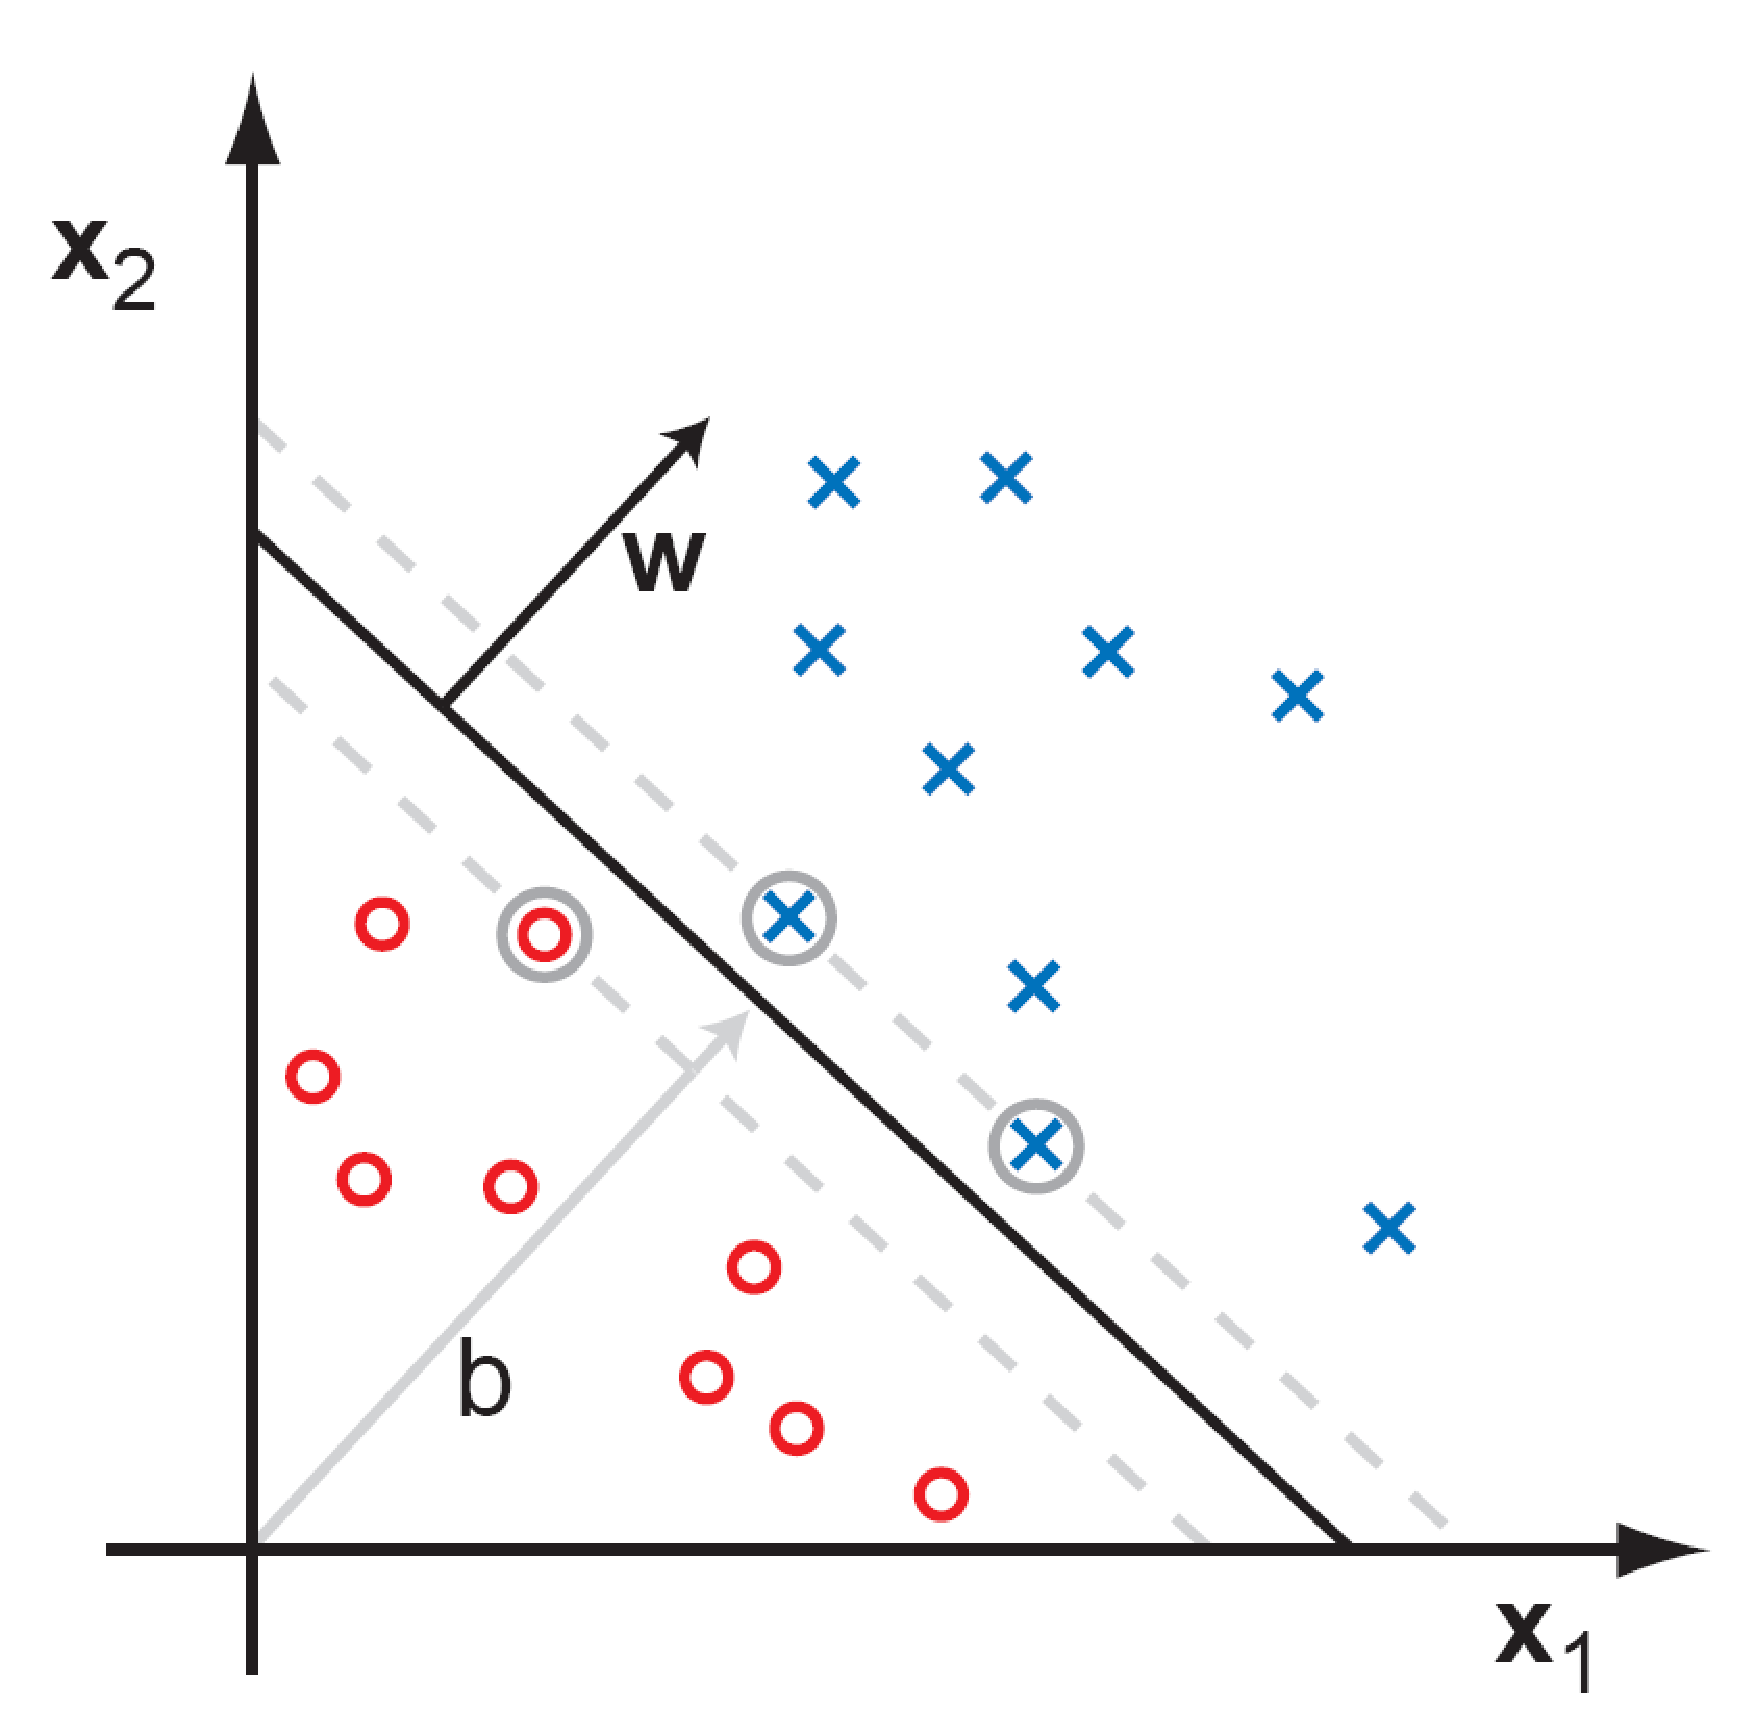
\includegraphics[scale=0.25]{images/svms-1-basic-2}
\par\end{centering}

\caption{The red circles and blue x's are the training data, the red circles
for the $y_{i}=-1$ class and the blue x's for the $y_{i}=+1$ class.
The data inside the grey circles are the support vectors that maximize
the distance between the data and the hyperplane defined by $w$,
a normal vector to the hyperplane and the offset $b$}

\end{figure}


Where $x$ is an input vector, $w$ is the weight vector, normal to
the separation hyperplane, and $b$ is the offset or bias:

\begin{eqnarray*}
 & w^{T}x+b\geq0\mbox{\,\,\,\,\,\,\,\,\,\,\,\,\,\,\,\,\,\,\,\,\,\,\,\,\,\,\,\,\,}for\,\,\,\,\,\,\, y_{i}=+1\\
 & w^{T}x+b<0\mbox{\,\,\,\,\,\,\,\,\,\,\,\,\,\,\,\,\,\,\,\,\,\,\,\,\,\,\,\,\,}for\,\,\,\,\,\,\, y_{i}=-1\end{eqnarray*}


For a given vector $w$ and offset $b$ the distance between the the
hyperplane defined in and a point $x$ is called margin of separation
represented by the equation\ref{eq:}.

Then we can write the discriminant function:

\begin{equation}
{g(x)=w}^{T}x+b\label{eq:2}\end{equation}


An the classification function as:

\begin{equation}
y=sign\{w^{T}x+b\}\label{eq:3}\end{equation}


Equation \ref{eq:2} gives a measure of the distance from x to the
optimal hyperplane, and \ref{eq:3} assign a category for a specific
point. 

As described above, the complexity of the classifier should be minimized
in order to achieve a good generalization, for linear classifier this
equivalent lowering that complexity is to maximize the margin of separation
between the points and the hyperplane. An approach to find this separator
is to maximize the margin between two parallel supporting planes,
if we define the margin as follows:

\begin{eqnarray*}
 & w^{T}x+b=\,\,\,1\\
 & w^{T}x+b=-1\end{eqnarray*}


Then the margin of separation is equal then to $\gamma=\frac{2}{w}$
. Now our problem becomes maximize $\frac{2}{w}$ which is equivalent
to minimize $||w||_{2}/2$ in the following quadratic programming
problem:

\begin{eqnarray}
 & \underset{w,b}{min} & \frac{1}{2}||w||^{2}\nonumber \\
s.t &  & y_{i}(w^{T}x_{i}+b)\geq1\label{eq:min0.5w2}\end{eqnarray}


Condition $d_{i}(w^{T}x_{i}+b)\geq1$ specify that all the data points
have to be classified correctly. In order to solve this problem we
introduce the Lagrangian formulation:

\-\begin{eqnarray}
\,\underset{\alpha}{max}\,\underset{w,b}{min}\,\, J(w,b,\alpha) & = & \frac{1}{2}w^{T}w-\sum_{i=1}^{N}\alpha_{i}[y_{i}(w^{T}x_{i}+b)-1]\label{eq:lagrangian}\\
s.t &  & \alpha_{i}\geq0\nonumber \end{eqnarray}


Now the conditions of optimality for $J(w,b,\alpha)$ are given by:

\begin{equation}
\,\,\,\,\,\frac{\delta J(w,b,\alpha)}{\delta w}=0\longrightarrow w=\sum_{i=1}^{N}\alpha_{i}y_{i}x_{i}\label{eq:weqsumadx}\end{equation}


\begin{equation}
\frac{\delta J(w,b,\alpha)}{\delta b}=0\longrightarrow\sum_{i=1}^{N}\alpha_{i}y_{i}=0\label{eq:sumadeq0}\end{equation}


Replacing \ref{eq:weqsumadx} and \ref{eq:sumadeq0} into \ref{eq:lagrangian}
and defining the cost function as $J(w,b,\alpha)=Q(\alpha)$ yields:

\begin{eqnarray}
min\, Q(\alpha) & = & \sum_{i=1}^{N}\alpha-\frac{1}{2}\sum_{i=1}^{N}\sum_{j=1}^{N}\alpha_{i}\alpha_{j}y_{i}y_{j}x_{i}^{T}x_{j}\label{eq:minq}\\
s.t &  & \alpha_{i}\geq0\,\, and\,\,\,\sum_{i=1}^{N}\alpha_{i}y_{i}=0\nonumber \end{eqnarray}


Which is a quadratic programming problem (QP). Notice that the dual
problem is cast entirely in terms of the training data. The fact that
this is a QP problem is one of the strength of this methodology and
also a weakness. It's a strength because as opposed to others techniques
such as Neural Networks, the optimization problem is convex and a
global optimum is always reached in a finite amount of time \cite{Joachims98}.
On the other hand, a QP is a computationally expensive problem, this
property has led to the development of both, novel ways of solving
the problem described in equation \ref{eq:minq} and alternative formulations
for solving the same optimization problem \cite{Suykens-et-al2002,Joachims/06a},
with varying degrees of performance. The $x{}_{i}$'s whose $\alpha{}_{i}$
are not defines are the support vectors, that is they are on the hyperplanes
that defines the maximum margin separator.

When all points cannot be shattered by one Hyperplane an error bound
is added in the form of a non negative slack variable, the primal
problem described in \ref{eq:min0.5w2} becomes:

\begin{eqnarray}
 & \underset{w,b}{min} & \frac{1}{2}||w||^{2}+C\sum_{i=1}^{N}\xi_{i}\nonumber \\
 &  & y_{i}(w^{T}x_{i}+b)+\xi_{i}\geq1\label{eq:min0.5w2plusc}\\
s.t\nonumber \\
 &  & \xi_{i}\geq0\,\,\,\, i=1,...,m\nonumber \end{eqnarray}


Where $C$ is a user-specified positive parameter and depends on the
data, empirical ways of finding the adequate C exist. After following
a similar procedure to the one that lead us to \ref{eq:minq} we now
have:

\begin{eqnarray}
min\, Q(\alpha) & = & \sum_{i=1}^{N}\alpha-\frac{1}{2}\sum_{i=1}^{N}\sum_{j=1}^{N}\alpha_{i}\alpha_{j}y_{i}y_{j}x_{i}^{T}x_{j}\nonumber \\
s.t\nonumber \\
 &  & \alpha\geq0\nonumber \\
 &  & \sum_{i=1}^{N}\alpha_{i}y_{i}=0\label{eq:minwithc}\\
 &  & 0<\alpha_{i}\leq C\,\,\,\, i=1,...,m\nonumber \end{eqnarray}


The C parameter defines the error bound, and in plain words in states
how {}``hard'' the classifier should try to correctly classify a
given point before removing it from the training set. Once calculated
the $\alpha_{i}$ the optimal weight vector $w_{o}$ and offset $b_{o}$
can be calculated as follows:

\begin{eqnarray}
 & w_{o}= & \sum_{i=1}^{N}\alpha_{i}y_{i}x_{i}\nonumber \\
\label{eq:w0b0}\\ & b{}_{o}= & 1-w_{o}^{T}x^{(s)}\nonumber \end{eqnarray}


Where $x^{(s)}$ is any support vector. We can also write the discriminant
function as follows:

\[
y=sign\{\sum_{i=1}^{N}d_{i}\alpha_{i}x_{i}^{T}x+b_{0}\}\]


Many times a linear separator is not enough to classify the data properly,
geometrically speaking, a more complex surface is needed in order
to separate the data correctly. In order to classify the data a non-liner
mapping into a high-dimensional feature space where the data is linearly
separable, the Cover's theorem on separability \cite{Cover65a|citeulike:1803784}
supports this procedure . in order to accomplish this, SVM uses the
so called {}``Kernel Trick'' which consist in the usage of a Kernel
function that maps the input data into a higher dimensional space.
The reader may consult the appropriate literature \cite{citeulike:368926|Haykin1998,citeulike:755348|Heibrich2001Lkernel,citeulike:114719|Cristianini2000introSVM}
for more information on this method. The dual for formulation using
this approach is:

\begin{eqnarray}
min\, Q(\alpha) & = & \sum_{i=1}^{N}\alpha-\frac{1}{2}\sum_{i=1}^{N}\sum_{j=1}^{N}\alpha_{i}\alpha_{j}d_{i}d_{j}K(x_{i},x_{j})\nonumber \\
s.t\nonumber \\
 &  & \alpha\geq0\nonumber \\
 &  & \sum_{i=1}^{N}\alpha_{i}d_{i}=0\label{eq:minwithckernel}\\
 &  & 0<\alpha_{i}\leq C\,\,\,\, i=1,...,m\nonumber \end{eqnarray}


And the discriminant function is:

\[
y=sign\{\sum_{i=1}^{N}d_{i}\alpha_{i}K(x_{i},x)+b_{0}\}\]


There are many available Kernel functions, and they depend on the
characteristics of the input data. In this work we are going to use
a linear SVM as defined in equation \ref{eq:minwithc}, which also
can be viewed as \ref{eq:minwithckernel} equation using the kernel
function: $K(x_{i,}x_{j})=x_{i}^{T}x_{j}$. 


\section{SVM and Text Categorization}

The usage of SVM was first introduced by Joachims \cite{Joachims98,Joachims99c}
and similar setups have been used in posterior literature\cite{DumaisPHS98}.
the TC task using SVM can bee seen geometrically as finding an hyperplane
(decision surface) that separates two groups of points. Each point
is a vector representation of a document which can be done using any
of the models described back in section \ref{sub:Models-of-Text}.
As argued by Joachims \cite{Joachims98}, SVMs offer two important
advantages for TC:

\begin{itemize}
\item Doing term selection is generally not needed, because SVM are robust
to overfitting problems and can scale up to high dimensions.
\item No human and machine effort in parameter tuning on a validation set
is needed, as there is a theoretical default choice of parameter settings.
\end{itemize}
These two characteristics makes the SVMs attractive for tackling this
kind of problems. In real life scenarios, TC problems involves high
dimensional data and large amount of computing processing. As mentioned
before, the fact that SVM need a lot of calculation power for training
makes it an important motivation for using a parallel algorithm when
training SVM.


\section{Transductive Learning for SVM\label{sub:Transductive-Learning-for}}

So far with the formulations described in the last section we are
using what is called inductive learning, in other words we start from
a set of examples, and based on them we try to find a classificator
function that classifies correctly the data. This is called Inference
learning, that is, going from particular examples to a general hypothesis.
The Transductive setting on the other hand, tries to use the known
distribution of the test data in order produce a classifier. 

This setting has a clear application when we don\textquoteright{}t
care about the particular function; we only need to classify a given
set of examples (i.e test set) with as few errors as possible. The
Transductive inference uses the training examples previously labeled
and the unclassified examples to generate an optimal partition and
labeling of the unclassified examples, using the prior knowledge provided
by the distribution of the unclassified examples.

The goal of the TSVM or Transductive learner is to select a function
$hL=L(S_{train},S_{test})$ from the hypothesis space $H$ using $S_{train}$
and $S_{test}$ such that the expected number of erroneous predictions
on the test and the training samples is minimized. But, why not use
the learning rule obtained by means of the training examples to classify
the test examples? The problem arises when a small training set is
use. The classifier will have a \textquotedblleft{}poor\textquotedblright{}
generalization due to the lack of knowledge about the distribution
of points in the space $X$ \cite{EspinosaJ2003}. 

The classifier function estimated with very few points will lead to
disappointing results. Unlike of the inductive setting, the Transductive
setting uses the location of the test examples when defining the structure.
Such structure corresponds to a structure of possible hypothesis solution.
Using prior knowledge about the nature of testing data provides extra
information to built an appropriate structure. The structure is build
based on the margin on both the training and the test data.

%
\begin{figure}[H]
\begin{centering}
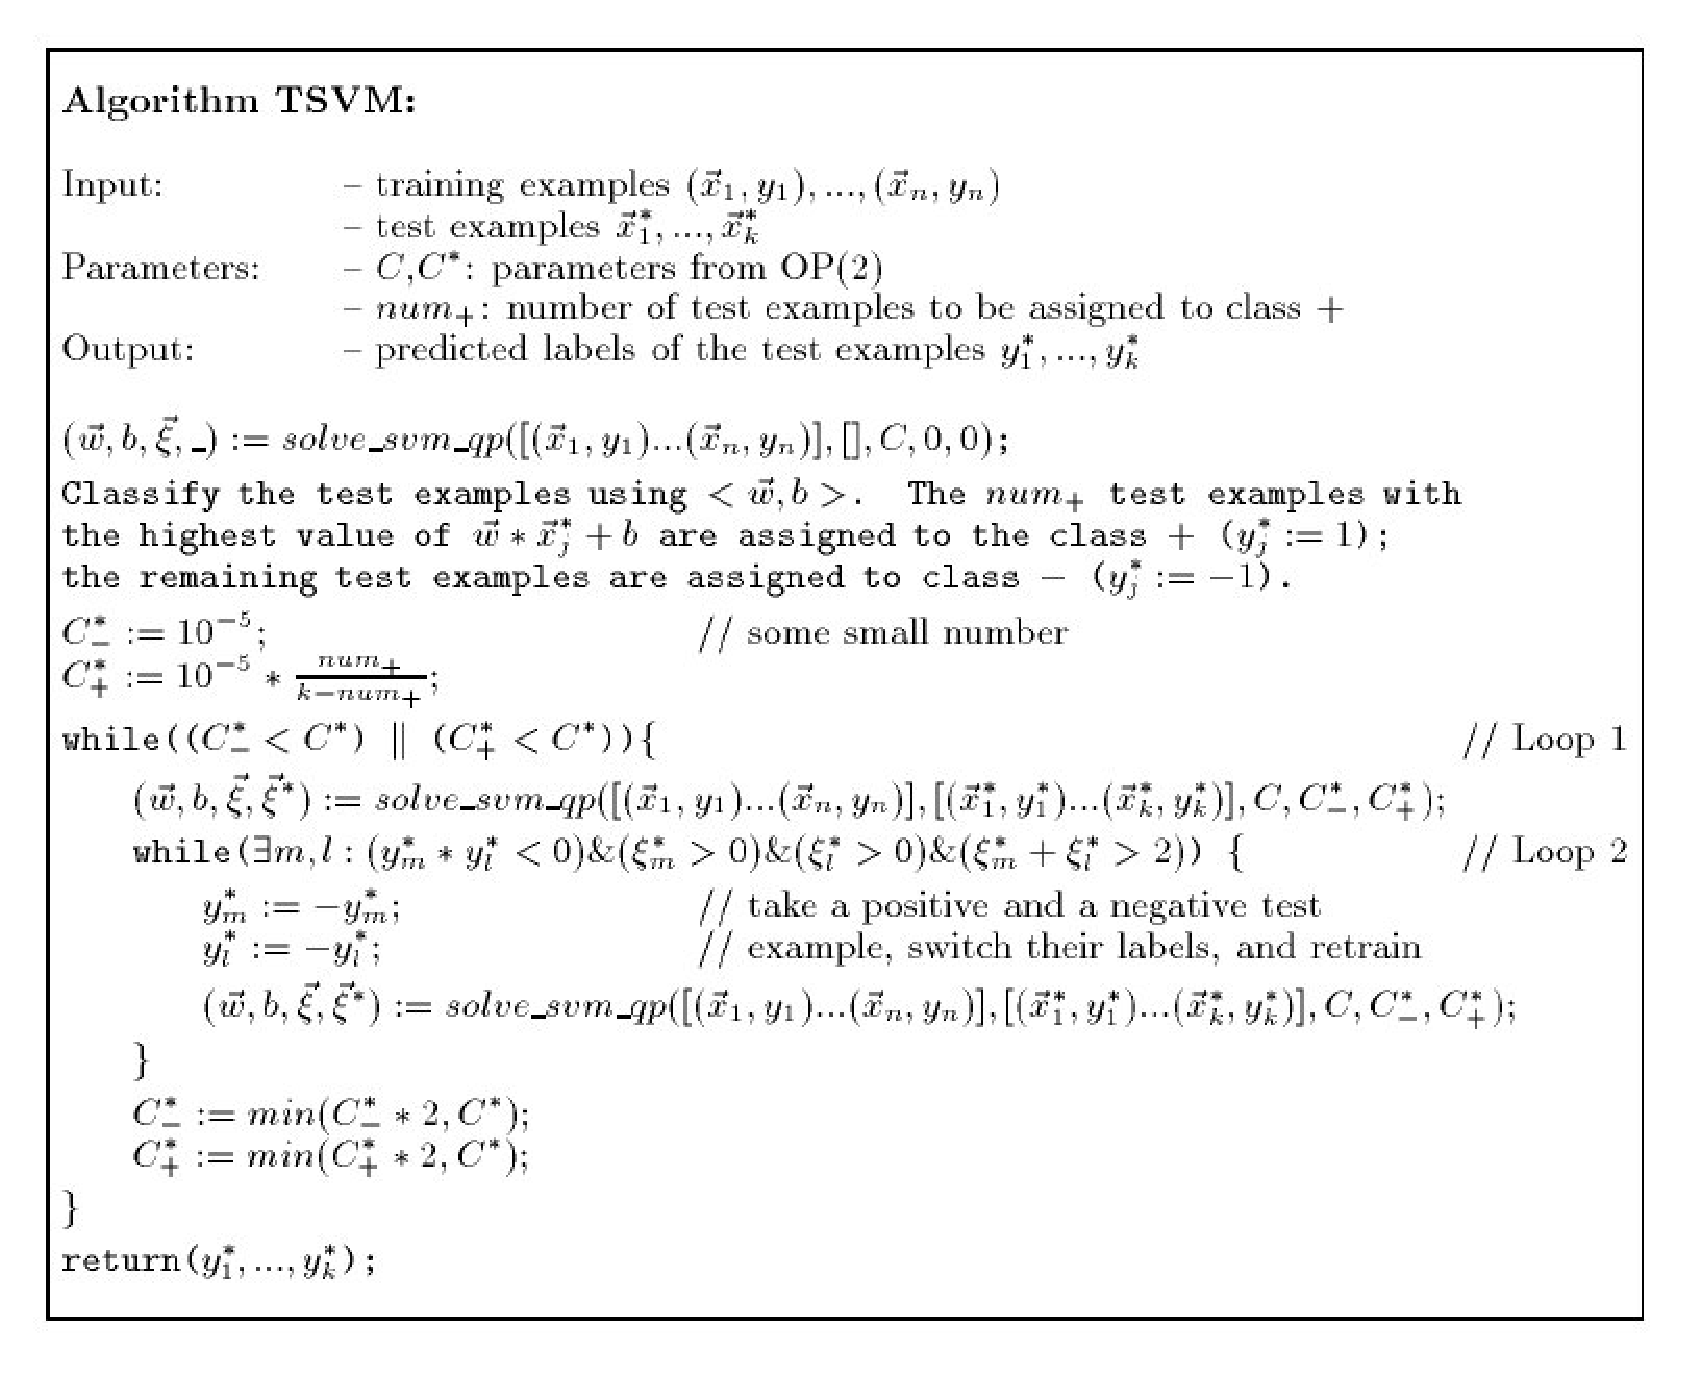
\includegraphics[scale=0.42]{images/joachims-algorithm}\label{fig:alg-tsvm}
\par\end{centering}

\caption{Algorithm for training Transductive Support Vector Machines \cite{Joachims99c}}



\end{figure}


{[}TODO Description of the algorithm] For a complete description and
a in depth study of the Joachims' approach see the nominal paper \cite{Joachims99c}
and work of Collobert \cite{1248609}.


\chapter{Parallel Methods for Training Transductive SVM \label{cha:Experiments-and-Results}}


\section{Introduction}

Solving the Transductive SVM using the algorithm described by Joachims
implies solve many times an SVM inductive optimization problem. The
algorithm improves the objective function by switching the labels
interactively of two unlabeled data points $x_{i}$ and $x_{j}$ with
$\xi_{i}+\xi_{j}>2$. It uses two nested loops to optimize a TSVM
which solves a quadratic programming every time it changes a label
from an unlabeled data. The convergence of the nested loop relies
in the fact that there is only a finite number $2^{U}$ ways of labeling
of $U$ unlabeled points and it is unlikely that all of them are examined
\cite{1248609}. However because the heuristic only swaps the label
of two unlabeled examples at each nested loop iteration it might need
(and in fact it does) many iterations to reach a minimum which makes
it intractable for big data sets in practice.

TSVM in the worst case have complexity of $O(L+U)^{3}$ with $U$
labeled points, although it generally scales to square in most practical
cases \cite{Joachims/99a} thus still intractable for large data sets.

In order to optimize this kind problem one can try to modify the formulation,
for instance example solving it in the primal rather than in the dual
with an alternate technique although the question of how widely applicable
are these methods are remains to bee seen. or use any of the general
approaches described in section \ref{sec:Paralell-Machine-Learning}
that makes use of the computation power given by the new multicore
processors. 

For the specific case of SVM and TSVM one could try to modify the
problem in a way that makes it easily parallelizable \cite{1248601}
Generally this is accomplished through the use of decomposition technique
of some kind. Another approach is to use a mixture of SVM \cite{citeulike:935557|Collobert2002}
in order to to train each of them with a subset and them using the
mixture of expert approach \cite{Jacobs:Jordan:Nowlan:Hinton91} which
is easily parallelizable. All these approach modify in some manner
the original formulation of the problem.

A recent approach called the Cascade SVM consist in an array of SVM
solvers arranged in pyramid form. This structure allows an easy parallelization
and does not modify the original formulation at all \cite{GrafCBDV04,ZhangZY05}.
This is the approach selected for the parallelization of TSVM because
there is no need to modify the original quadratic programming problem
and is straightforward to implement. Some small modifications are
needed in order to be fully adapted to the Transductive algorithm
described by Joachims. 


\section{The Cascade SVM}

The Cascade SVM was described by Graf et al \cite{GrafCBDV04} and
further explored by Zhang et al \cite{ZhangZY05} and is based in
the strategy of early elimination of non-support vectors from the
training set \cite{Joachims/99a}. The Cascade SVM is a distributed
architecture where smaller optimization problems are solved independently
making them easily parallelizable. The results of this smaller problems
are then assembled in a way that is ensured that it eventually converges
to globally optimal solution.

%
\begin{figure}[H]
\begin{centering}
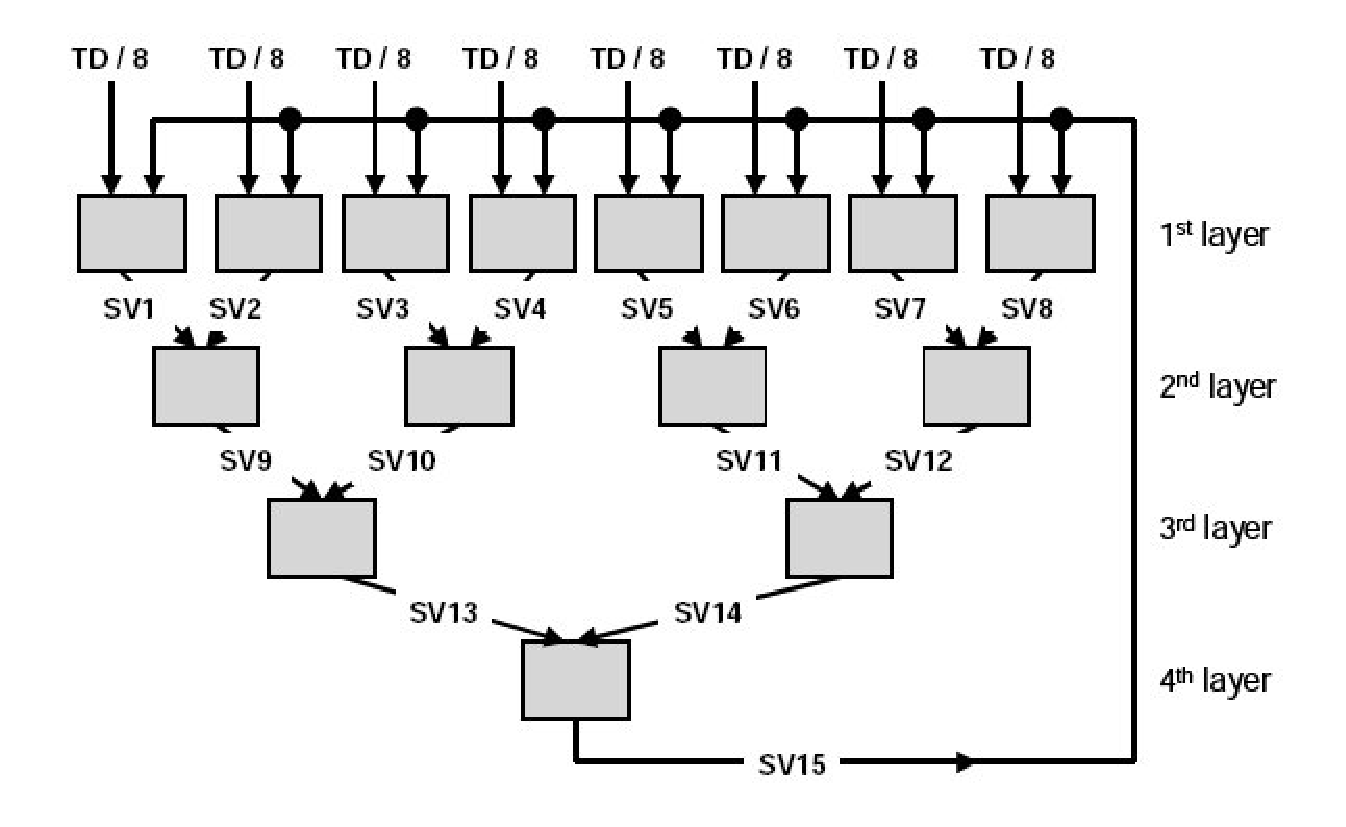
\includegraphics[scale=0.5]{images/graf-svm-cascade}
\par\end{centering}

\caption{Schematic of a Cascade architecture \cite{GrafCBDV04}}
\label{fig:svm-cascade}
\end{figure}


In order to find a minimum using this approach the problem is initialized
with a number of independent smaller optimization whose results are
combined in later stages in a hierarchical fashion as shown in figure
\ref{fig:svm-cascade}. The data is split into subsets and everyone
of them is evaluated for to find support vectors in the first layer,
then the results are combined two-by-two and entered as training set
for the next layer. Often a single pass through the cascade produces
satisfactory results and if it is not the case, that is, if solution
is not the global maximum, the result of the last layer is fed back
into the first layer, where each of the SVM of the first layer receives
all the support vectors and test them with fraction of his inputs
to check if any of them have to be incorporated into the optimization.
If this is not the case for all SVM of the input layer, the cascade
have converged otherwise it proceeds with another pass through the
network. The formal proof of the convergence can be found in \cite{GrafCBDV04}.


\subsection{Cascade Transductive SVM}

The original formulation for this cascade SVM is defined for the classical
SVM problem so it is necessary to adapt the architecture described
above in order to handle properly the TSVM formulation. There are
at least two approach for this, the first approach is to make each
of theSVM in the array Transductive, using the algorithm described
in Figure \ref{fig:alg-tsvm}. Even if this might seem obvious ultimatly
the loop in each of the SVM will be run in just one processor so the
only possible speed up would be in terms of the number of training
and testing data available. Also splitting and mergin the subsets
might need additional modifications, despite this fact, it might be
interesting to vizualise the behaviour of this approach and for that
reason is left as a future work.

The other approach is parallelize the more computational expensive
part of the TSVM algorithm: the \emph{solve\_svm\_qp} function which
solves the dual problem associated with formulation described in section
\ref{sub:Transductive-Learning-for}. Now for each iteration of the
loop the a SVM inductive problem is solved in a parallel manner. We
have two goals to achieve with this, in the first place we need to
implement an algorithm that is at least is as good as the serial (non
parallel) version and also we need to ensure a speed up of the process
through the use of the parallel architecture.


\subsection{Merging Data Sets for the Transductive Case}

%
\begin{figure}
\begin{centering}
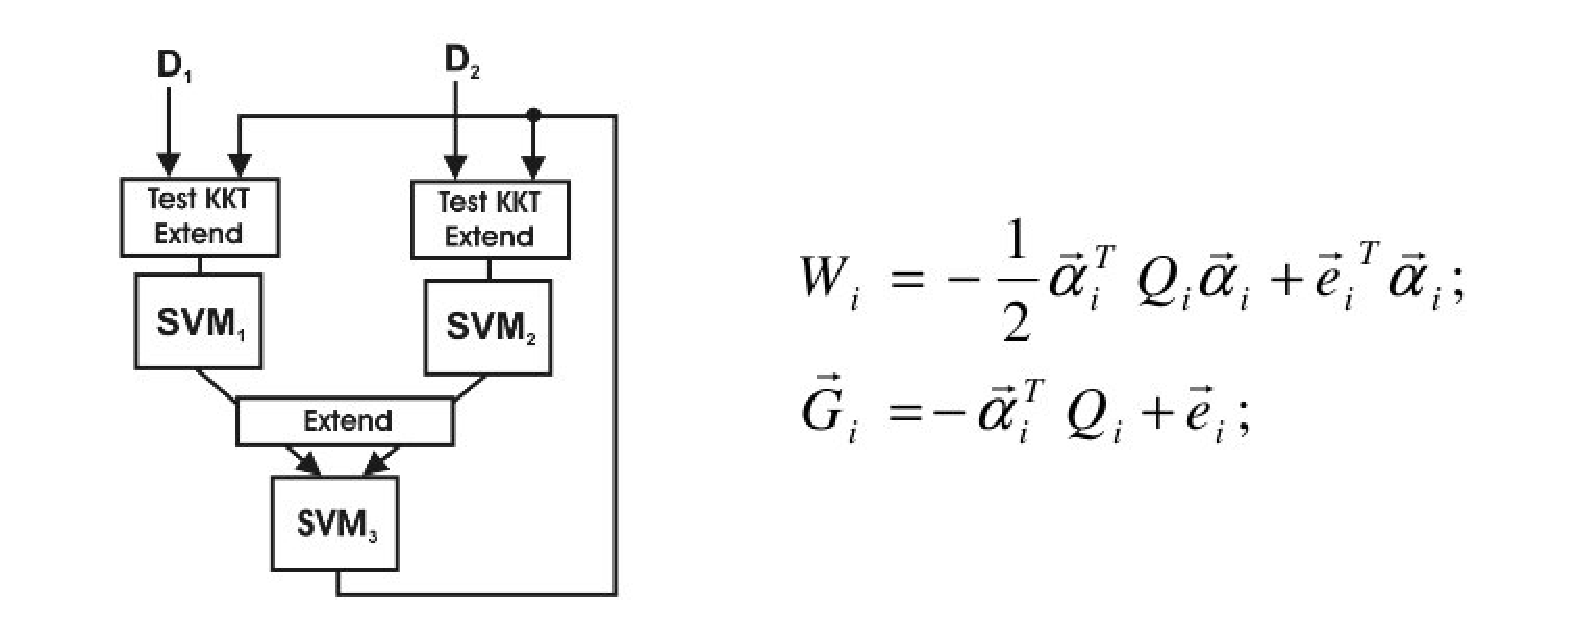
\includegraphics[scale=0.5]{images/graf-svm-cascade-of-3}\label{fig:graf-3-svm}
\par\end{centering}

\begin{centering}
\caption{A Cascade with two input sets $D_{1}$,$D_{2}$. $W_{i}$, $G_{i}$
and $Q_{i}$ are objective function, gradient, and kernel matrix,
respectively, of \noun{SVM}$_{i}$ (in vector notation); Gradients
of \noun{SVM}$_{1}$ and \noun{SVM}$_{2}$ are merged as indicated
in \ref{eq:mergin-subsets} and are entered into \noun{SVM}$_{3}$.
\cite{GrafCBDV04}}

\par\end{centering}
\end{figure}


In this section it is described the procedure to merge two subsets
using as example the description in the figure \ref{fig:graf-3-svm}.
For Transductive SVM there is not practically any change besides that
when recreating creating the problem for \noun{SVM}$_{3}$ we have
to take into account two boundaries for the values of $\alpha_{i}$
instead of one: $C$ for $\{a_{1}...\alpha_{L}\}$and $C*$ for $\{a_{L+1}...\alpha_{L+U}\}$.
Also, the process of elimination of early non-support vector machine
that is made on both groups, the labeled and the unlabeled data. 

The starting point and gradient for the merged set are defined below:

\begin{eqnarray}
 & W\, & =\frac{1}{2}\left[\begin{array}{c}
\vec{\alpha_{1}}\\
\vec{\alpha}_{2}\end{array}\right]^{T}\left[\begin{array}{cc}
Q_{1} & Q_{12}\\
Q_{21} & Q_{2}\end{array}\right]\left[\begin{array}{c}
\vec{\alpha_{1}}\\
\vec{\alpha}_{2}\end{array}\right]+\left[\begin{array}{c}
\vec{e_{1}}\\
\vec{e}_{2}\end{array}\right]^{T}\left[\begin{array}{c}
\vec{\alpha_{1}}\\
\vec{\alpha}_{2}\end{array}\right]\nonumber \\
\label{eq:mergin-subsets}\\\nonumber \\ &  & \vec{G_{3}=}\left[\begin{array}{c}
\vec{\alpha_{1}}\\
\vec{\alpha}_{2}\end{array}\right]^{T}\left[\begin{array}{cc}
Q_{1} & Q_{12}\\
Q_{21} & Q_{2}\end{array}\right]+\left[\begin{array}{c}
\vec{e_{1}}\\
\vec{e}_{2}\end{array}\right]\nonumber \end{eqnarray}


With $Q_{12}=Q_{1}Q_{2}$ and $Q_{21}=Q_{2}Q_{1}$. 

One thing that should be noted is the error values handling. As the
reader can see in \ref{fig:alg-tsvm} the decision whether to swap
the values of the labels for each uncategorized data depends on the
error of the classification of that particular value but as in each
layer we eliminate them in the process, we have to keep a record of
the classification error of the eliminated unlabeled vector because
we are going to use in the decision of the second loop.


\chapter{Experiments and Results}

In this section we present the experimental results for text classification
task. The base algorithm and auxiliary routines were programmed in
Matlab 7.4%
\footnote{http://www.mathworks.com/%
} using the Matlab \emph{quadprog} function which is a convex QP solver.
In order to fully parallelize the Cascade Architecture we made use
of the Distributed Computer Tool Box which enabled us to run the algorithm
in all the cores available. For the experiments we used a Desktop
computer with Processor Intel$^{\textregistered}$ Pentium$^{\textregistered}$
Dual Core CPU 3.40GHz with 1.5 GB of RAM.

For the experiments we use a subset of the 20 Newsgroups \cite{20news}
data set found in the UCI ML Repository\cite{Asuncion+Newman:2007}.
The data set was preprocessed using English stop-words and the Porter
stemmer algorithm \cite{Porter80} in a similar fashion as described
in section \ref{sub:Feature-Selection-and} and the feature vectors
were created using the \emph{tf-idf} formula. The code was written
in Ruby using an already existing implementation of the stemmer algorithm. 


\section{Experiments}

The 20 Newsgroup data sets is set is a collection of approximately
20,000 newsgroup documents, partitioned evenly across 20 different
newsgroups. The collection is organized in the following form:\\ 

\begin{tabular}{|c|c|c|}
\hline 
%
\begin{minipage}[t][1\totalheight][c]{0.33\columnwidth}%
\begin{itemize}
\item comp.graphics 
\item comp.os.ms-windows.misc
\item comp.sys.ibm.pc.hardware 
\item comp.sys.mac.hardware 
\item comp.windows.x\\ 
\end{itemize}
%
\end{minipage} & %
\begin{minipage}[t][1\totalheight][c]{0.27\columnwidth}%
\begin{itemize}
\item rec.autos 
\item rec.motorcycles 
\item rec.sport.baseball 
\item rec.sport.hockey
\end{itemize}
%
\end{minipage} & %
\begin{minipage}[t][1\totalheight][c]{0.27\columnwidth}%
\begin{itemize}
\item sci.crypt 
\item sci.electronics 
\item sci.med sci.space
\end{itemize}
%
\end{minipage}\tabularnewline
\hline 
%
\begin{minipage}[t][1\totalheight][c]{0.33\columnwidth}%
\begin{itemize}
\item misc.forsale
\end{itemize}
%
\end{minipage} & %
\begin{minipage}[t][1\totalheight][c]{0.27\columnwidth}%
\begin{itemize}
\item talk.politics.misc 
\item talk.politics.guns 
\item talk.politics.mideast
\end{itemize}
%
\end{minipage} & %
\begin{minipage}[t][1\totalheight][c]{0.27\columnwidth}%
\begin{itemize}
\item talk.religion.misc 
\item alt.atheism 
\item soc.religion.christian
\end{itemize}
%
\end{minipage}\tabularnewline
\hline
\end{tabular}

.\newline

As we can see the data set is divided by newsgroup topics and can
be grouped into similar categories. For the experiments we define
two tasks, an {}``easy'' one and an {}``hard'' one. For the easy
task we took 1000 messages from \emph{alt.atheism }and 1000 messages
from \emph{comp.graphics}. We call this an easy task because the terms
that appear in the documents from each collection are different, so
we can expect a nearly separable problem. The hard task we chose related
news groups were is expected that the most important terms similar
for both collection. We chose c\emph{omp.sys.ibm.pc.hardware} and
\emph{comp.sys.mac.hardware }for evaluating the SVM effectiveness
and computation times with also 1000 messages from each of them. The
data was split in a training set (20\%) and testing or ulabeled set
(80\%). The unlabeled set for the TSVM was used as the testing set
for the classic SVM. We also made some test with fewer training data
but with the same amount of test data in order to visualize better
the goods of transductive inference when only few training data is
available.

As performance measure we chose $F1$ as measure of effectiveness,
we also show the values of precision and recall for the experiments.
The kernel choice for the SVM was the linear kernel which has been
reported to be effective for text categorization tasks \cite{Joachims99c,DumaisPHS98},
thanks in part to the high dimensional nature of the input vectors.
The $C$ parameter was estimated for the two sets using 5-fold cross
validation with the training set. The other parameter defined by Joachim's
algorithm is $num+$, the number of test inputs to be labeled initially
as positive, in our implementation this number is also half of the
total test set, thus ensuring the precision and recall break-even.
The choice of the parameter $C*$is done using many heuristics, however
we use the one proposed by Joachims which consists in making it equal
to $C$. This parameter is of great importance for the computation
time of the overall algorithm because the annealing used by Joachim's
algorithm, for that reason we wanted to improve the computation time
by choosing the right C{*} parameter so we tested the implementation
effectiveness with the original Joachim's heuristic $C=C*$. %
\begin{comment}
and the one proposed by \cite{1248609}: $UC=LC*$ . 
\end{comment}
{}

The Cascade architecture used in the experiments were formed 3 layers
of SVM with 4 SVMs in the first 2 in the second and finally 1 in the
last layer.

Besides the categorization performance, we are interested in the computation
time, we expect that with the appropriate formulation of the parallel
architecture, reduce the impact of the computation time of the TSVM
Algorithm.


\subsection{Toy Experiment}

With the objective of prove the methods and their performance, a test
with few training and test samples was carried out first, the number
of features is also less than the full problem formulation because
only a fraction of these were preprocessed for this initial test.
For this toy experiments the hard task was performed with 200 testing
messages, 100 from c\emph{omp.sys.ibm.pc.hardware }labeled positive
and 100 from \emph{comp.sys.mac.hardware }labeled negative. The training
set consisted also of 200 messages with the same characteristics.
In these experiments (Table \ref{tab:Toy-Experiment:-comp.sys.ibm.pc.hardware})
the number of training samples varies for each test so we can appreciate
the difference in the performance of the methods. T stand for number
of training samples and S for number of testing samples. We can appreciate
that transduction algorithm perform much better than inductive when
few training samples, a very attractive characteristic for many real
problems. Even when the number of training samples is equal to the
number of testing samples the transductive outperforms the inductive
algorithm for the F measure.

%
\begin{table}[H]
\begin{tabular}{cc}
\begin{tabular}{|c|c|c|c|}
\hline 
T: 30 S: 200 & $P$  & $R$  & $F1$ \tabularnewline
\hline
\hline 
SVM & 0.44 & 0.8148 & 0.5714\tabularnewline
\hline 
TSVM & 0.7 & 0.7 & 0.7\tabularnewline
\hline 
TSVM Parallel & 0.7 & 0.7 & 0.7\tabularnewline
\hline
\end{tabular} & \begin{tabular}{|c|c|c|c|}
\hline 
T: 100 S: 200 & $P$  & $R$  & $F1$ \tabularnewline
\hline
\hline 
SVM & 0.94 & 0.7581 & 0.8393\tabularnewline
\hline 
TSVM & 0.84 & 0.84 & 0.84\tabularnewline
\hline 
TSVM Parallel & 0.84 & 0.84 & 0.84\tabularnewline
\hline
\end{tabular}\tabularnewline
 & \tabularnewline
\begin{tabular}{|c|c|c|c|}
\hline 
T: 200 S:200 & $P$  & $R$  & $F1$ \tabularnewline
\hline
\hline 
SVM & 0.94 & 0.7666 & 0.8624\tabularnewline
\hline 
TSVM & 0.87 & 0.87 & 0.87\tabularnewline
\hline 
TSVM Parallel & 0.87 & 0.87 & 0.87\tabularnewline
\hline
\end{tabular} & \tabularnewline
\end{tabular} 

\caption{Small Scale Experiment: \emph{comp.sys.ibm.pc.hardware} and\emph{
comp.sys.mac.hardware} with 200 messages from each newsgroup. \label{tab:Toy-Experiment:-comp.sys.ibm.pc.hardware}}

\end{table}





\subsection{Easy Task}

As mentioned above the easy task is an experiment were is expected
a linear separable problem formed by messages from newsgroups with
very disjoint topics. The number of features for each vector was 30854,
a high dimensional problem the with the parameter C = 10 from the
5-fold cross validation. Table \ref{tab:Easy-Task:comp.graphics-and}
shows the results of the experiments. 

%
\begin{table}
\begin{longtable}{c}
\begin{tabular}{|c|c|c|c|c|c||c|}
\hline 
 & \#Labeled & \#Unlabeled & $P$  & $R$  & $F1$  & Time (min)\tabularnewline
\hline
\hline 
SVM & 200 & N/A & 0.9245 & 1.0 & 0.9608 & 0.0137\tabularnewline
\hline 
TSVM & 200 & 200 & 0.9847 & 0.9847 & 0.9847 & 10.2205\tabularnewline
\hline 
TSVM Parallel & 200 & 200 & 0.9847 & 0.9847 & 0.9847 & \textcolor{red}{7.2050}\tabularnewline
\hline
\end{tabular}\tabularnewline
\tabularnewline
\begin{tabular}{|c|c|c|c|c|c||c|}
\hline 
 & \#Train & \#Unlabeled & $P$  & $R$  & $F1$  & Time (min)\tabularnewline
\hline 
SVM & 200 & N/A & 0.9384 & 1 & 0.9682 & 0.0135\tabularnewline
\hline 
TSVM & 200 & 400 & 0.9823 & 0.9823 & 0.9823 & 44.4103\tabularnewline
\hline 
TSVM Parallel & 200 & 400 & 0.9823 & 0.9823 & 0.9823 & \textcolor{red}{15.3406}\tabularnewline
\hline
\end{tabular}\tabularnewline
\tabularnewline
\tabularnewline
\begin{tabular}{|c|c|c|c|c|c||c|}
\hline 
 & \#Train & \#Unlabeled & $P$  & $R$  & $F1$  & Time (min)\tabularnewline
\hline 
SVM & 100 & N/A & 0.9062 & 1 & 0.9508 & 0.0135\tabularnewline
\hline 
TSVM & 100 & 400 & 0.9823 & 0.9823 & 0.9823 & 32.1135\tabularnewline
\hline 
TSVM Parallel & 100 & 400 & 0.9823 & 0.9823 & 0.9823 & \textcolor{red}{11.0953}\tabularnewline
\hline
\end{tabular}\tabularnewline
\tabularnewline
\begin{tabular}{|c|c|c|c|c|c||c|}
\hline 
 & \#Train & \#Unlabeled & $P$  & $R$  & $F1$  & Time (min)\tabularnewline
\hline
\hline 
SVM & 100 & N/A & 0.9975 & 0.8957 & 0.9438 & 0.0135\tabularnewline
\hline 
TSVM & 100 & 800 & 0.9798 & 0.9798 & 0.9798 & 214.2297\tabularnewline
\hline 
TSVM Parallel & 100 & 800 & 0.9798 & 0.9798 & 0.9798 & \textcolor{red}{68.4745 }\tabularnewline
\hline
\end{tabular}\tabularnewline
\tabularnewline
\begin{tabular}{|c|c|c|c|c|c||c|}
\hline 
 & \#Train & \#Unlabeled & $P$  & $R$  & $F1$  & Time (min)\tabularnewline
\hline
\hline 
SVM & 100 & 0 & 0.8966 & 0.9975 & 0.9444 & 0.0135\tabularnewline
\hline 
TSVM & 100 & 1600 & 0.9800 & 0.9800 & 0.9800 & 278.3236%
\begin{comment}
228.3235
\end{comment}
{}\tabularnewline
\hline 
TSVM Parallel & 100 & 1600 & 0.9800 & 0.9800 & 0.9800 & 41.53950\tabularnewline
\hline
\end{tabular}\tabularnewline
\end{longtable}

\caption{The {}``Easy'' Task:\emph{ comp.graphics} and \emph{alt.atheism}.
Using C=10 \label{tab:Easy-Task:comp.graphics-and} }

\end{table}


We can notice how the classical SVM algorithm is always faster that
the Transductive implementation and for this specific problem, which
is expected to be almost linear separable, with few unlabeled data
the classification performance is very similar, while the difference
in speed of the algorithm is really huge. However when the training
data decreases and more there is more unlabeled data the differences
in classification performance begin to be more noticeable, even with
this {}``easy'' problem. Regarding the speed, is obvious by the
results that that the standard SVC algorithm is by far faster than
its transductive counterparts, therefore we are going to discuss the
differences between the transductive and its parallel version. For
this problem, the classification performance of the transductive algorithms
were the same, thus one of the objectives was accomplished, to maintain
the same classification performance while performing the tasks in
parallel. Of course, the gains of the parallel approach and the early
eliminations of non-support vectors are devised in the time used for
the calculations on the Transductive SVM problem. One thing that can
be noticed in the tables is that the parallel version of the algorithm
no necessarily is slower when facing much more data, this is due to
the process of early elimination of non-support vector and it may
happen that with much more data more non-support vectors are eliminated
in proportion with the amount of unlabeled data, making the whole
process faster. This particular property can be really appealing when
working with larger datasets, of course it will depend entirely on
the dataset.


\subsection{Hard Task}

This is task is formed from 2000 messages from the categories of \emph{comp.sys.ibm.pc.hardware}
and\emph{ comp.sys.mac.hardware} which have many equal terms thus
making it a possible not linearly separable problem. The number of
features extracted for this problem is 26997. The parameter choice
for C = 9 and was taken from the same 5-fold cross-validation with
the available training data.

%
\begin{table}
\begin{longtable}{c}
\begin{tabular}{|c|c|c|c|c|c||c|}
\hline 
 & \#Train & \#Unlabeled & $P$  & $R$  & $F1$  & Time (min)\tabularnewline
\hline 
SVM & 100 & N/A & 0.7400 & 0.8916 & 0.8087 & 0.0025\tabularnewline
\hline 
TSVM & 100 & 200 & 0.8600 & 0.8600 & 0.8600 & 1.5370\tabularnewline
\hline 
TSVM Parallel & 100 & 200 & 0.8700 & 0.8700 & 0.8700 & 1.4863\tabularnewline
\hline
\end{tabular}\tabularnewline
\tabularnewline
\begin{tabular}{|c|c|c|c|c|c||c|}
\hline 
 & \#Train & \#Unlabeled & $P$  & $R$  & $F1$  & Time (min)\tabularnewline
\hline 
SVM & 100 & N/A & 0.8830 & 0.7550 & 0.8140 & 0.0025\tabularnewline
\hline 
TSVM & 100 & 400 & 0.8550 & 0.8550 & 0.8550 & 6.0628\tabularnewline
\hline 
TSVM Parallel & 100 & 400 & 0.8550 & 0.8550 & 0.8550 & 4.3323\tabularnewline
\hline
\end{tabular}\tabularnewline
\tabularnewline
\begin{tabular}{|c|c|c|c|c|c||c|}
\hline 
 & \#Train & \#Unlabeled & $P$  & $R$  & $F1$  & Time (min)\tabularnewline
\hline
\hline 
SVM & 100 & N/A & 0.7350 & 0.8724 & 0.7978 & 0.0025\tabularnewline
\hline 
TSVM & 100 & 800 & 0.8200 & 0.8200 & 0.8200 & 31.0015\tabularnewline
\hline 
TSVM Parallel & 100 & 800 & 0.8200 & 0.8200 & 0.8200 & 19.5472\tabularnewline
\hline
\end{tabular}\tabularnewline
\tabularnewline
\begin{tabular}{|c|c|c|c|c|c||c|}
\hline 
 & \#Train & \#Unlabeled & $P$  & $R$  & $F1$  & Time (min)\tabularnewline
\hline
\hline 
SVM & 100 & 0 & 0.7362 & 0.8624 & 0.7943 & 0.0135\tabularnewline
\hline 
TSVM & 100 & 1600 & 0.8187 & 0.8187 & 0.8187 & 221.5013\tabularnewline
\hline 
TSVM Parallel & 100 & 1600 & 0.8187 & 0.8187 & 0.8187 & 86.1924\tabularnewline
\hline
\end{tabular}\tabularnewline
\tabularnewline
\tabularnewline
\tabularnewline
\end{longtable}

\caption{The {}``Hard'' Task:\emph{ }of \emph{comp.sys.ibm.pc.hardware} and\emph{
comp.sys.mac.hardware}. Using C=9 \label{tab:Hard-Task:comp.graphics-and} }

\end{table}


As expected, the TSVM performed better than the classic linear SVM,
however due to the nature of the data, the classification performance
difference between the two the TSVM and the SVM was not really substantial.
Another thing to notice is that this example is somewhat counter-intuitive,
because you could expect that for more training data available the
difference between the classification performance between the classical
and the transductive SVM would increase. However the opposite happened,
when more training data was available, the difference between their
performance decreased. Another result of the experiment, that surprised
us but we knew it could happen was the for the 100-200 setup the transductive
parallel SVM had a little bit more classification performance than
the non-parallel version. Even with this particularities in general
terms the expected occurred, the classification performance of the
transductive setting was higher than the inductive one, and the parallel
version of the TSVM run almost 3 times faster than the non transductive
one.


\section{Conclusion And Future Direction}



In this work we have implemented a parallel version of TSVM as described
by Joachims' \cite{Joachims99c}, an approach that because its annealing
heuristics requires many iterations solving a similar problems. Our
approach, in order to speed up the process, was to parallelize the
SVM solver function using a Cascade architecture. We have shown that
this approach speed up the process 2 to 7 times using just one dual
core processor. This architecture scales very well, therefore is expected
that, with more processors available the the speed gains will be even
more noticeable. In addition, more layers in basic architecture could
help in the improvement of the computation time. 

From the data tables one could argue that the classification performance
gains for using TSVM does not worth the computation time spent even
with this parallel approach. However this last statement is in someway
subjective, as the trade-off between speed and classification performance
depends in nature of the problem, it would be possible that we would
prefer more classification performance at cost of computation time.
Also, if more and more processors/cores available (as it is the actual
trend) the speed gains could be much more noticeable. 

Regarding the classification performance of the TSVM algorithm we
noticed something particular, the best C for the C{*} for the transductive
setting does not generally match in the sense that the best C parameter
for the inductive problem does not produce the best classification
performance in the transductive problem for the given set of data.
However, we have chosen the parameter that works best for the inductive
setting.

However it is truth that more optimization strategies have to be developed
in order to make this algorithm really usable in real world situation.
Now, with a parallel and scalable version of the transductive algorithm
a series of strategies could be explored in order to further optimize
the computation time, however the implementation of such strategies
is outside the scope of this work and are mentioned here as a possible
future work.

Maybe the most obvious approach is that given that the data is split
in equal parts (subsets), and per each iteration only one of the parts
is modified (i the labels of two of the entries) there is not need
recalculate the other parts of the n and they can be reused. For example
in our particular case, we calculated 7 distinct SVM problems (as
our architecture o 3 layers t in 4-2-1 e respectively), using caching
we wold only need to calculate all of them once at the r and then
only when a pair of of vector fell of different SVM problem. For the
most of the iterations we would only need to calculate 3 problems. 

Another strategy would be try new improved heuristics as described
by Collobert et al \cite{citeulike:935557|Collobert2002} and modifying
in Joachims' TSVM by reducing iteration in the cycles or interchanging
more labels per iteration. This last is important because the annealing
heuristic used by Joachim's TSVM is source of the elevated computation
time.

A good thing about this approach is that any improvement to the SVM
formulation can be directly applied to the SVM, for example the technique
of Zanghirati et al. \cite{782654}could be applied to each one of
the SVM solvers in order to have multilevel parallelization, further
improving the computation performance.

\bibliographystyle{acm}
\bibliography{bibblio}

\end{document}
